% !TEX program = xelatex
\documentclass[11pt,aspectratio=169]{beamer}

\makeatletter
\def\@makefnmark{}
\makeatletter

\setbeamersize{text margin left=5mm,text margin right=5mm} 

\usepackage{amsthm,amsmath,amssymb,braket,fontspec}
\usepackage[absolute,overlay]{textpos}

\usetheme[numbering=none,nofirafonts]{focus}

\setbeamercolor{footnote}{fg=blue}
\setbeamerfont{footnote}{size=\small}
\setbeamertemplate{bibliography item}[triangle]

\setmainfont{Fira Sans}
\setsansfont{Fira Sans}
\setbeamerfont{title}{size=\LARGE, shape=\scshape}
\setbeamerfont{author}{size=\large, shape=\scshape}
\setbeamerfont{institute}{size=\normalsize, shape=\scshape}
\setbeamerfont{date}{size=\normalsize, shape=\scshape}
\setbeamerfont{frametitle}{size=\large, shape=\scshape}

\usepackage[backend=bibtex,url=false,doi=false,maxcitenames=1, style=authoryear]{biblatex}
\bibliography{local-mit}
\AtBeginBibliography{\scriptsize}

\newcommand{\focus}[1]{\textcolor{red}{#1}}

\definecolor{red}{HTML}{CC0000}
\setbeamertemplate{bibliography item}[triangle]

\AtBeginSection[]{
\begin{frame}
  \vfill
  \centering
  \begin{beamercolorbox}[sep=20pt,rounded=true,center]{frametitle}
    \usebeamerfont{title}\insertsectionhead\par%
  \end{beamercolorbox}
  \vfill
\end{frame}
}
\title{
{Local metal-insulator transition in an\\ extended Anderson impurity model}
}
\date{\today}
\author{Abhirup Mukherjee, Siddhartha Lal}
\institute{Department of Physical Sciences, IISER Kolkata, Mohanpur}
\date{\today}

\begin{document}

\centering

\begin{frame}
\maketitle
\begin{textblock*}{0.7\textwidth}(7.5cm, 6cm)
	\centering
	\vspace*{\fill}

	\hspace*{\fill}
	
\includegraphics[width=0.2\textwidth]{figures/epqm_logo_mod.jpeg}
	
\includegraphics[width=0.2\textwidth]{figures/dps_logo.jpeg}
	\hspace*{\fill}

	\vspace*{\fill}
\end{textblock*}
\end{frame}

\section{Why another impurity model?}

\begin{frame}{Anderson and Kondo impurity models - No transition!}

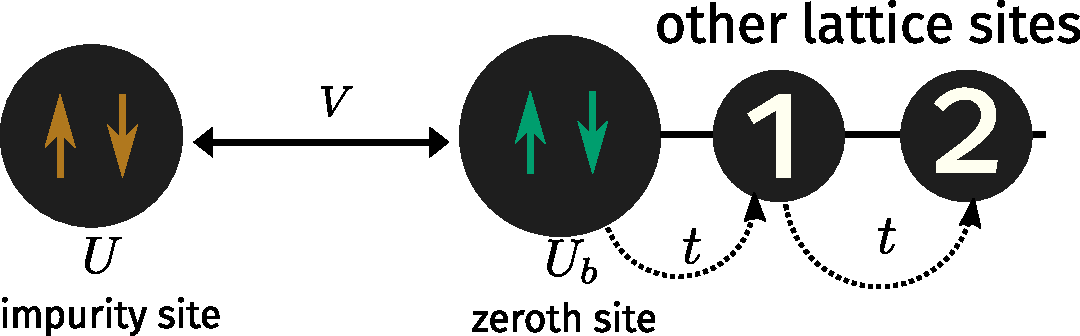
\includegraphics[width=0.6\textwidth]{figures/siam.pdf}

\vspace*{\fill}

\begin{itemize}
	\item simplest impurity models - Anderson and Kondo \\[10pt]
	\item localisation physics + hybridisation\\[10pt]
	\item impurity is \focus{screened} at low \(T\)
\end{itemize}

\footcite{anderson_1961,anderson_1978,kondo1964resistance,wilson1975,hrk_wilson_1980,andreiKondoreview}

\end{frame}

\begin{frame}{DMFT and the Mott MIT}
\centering

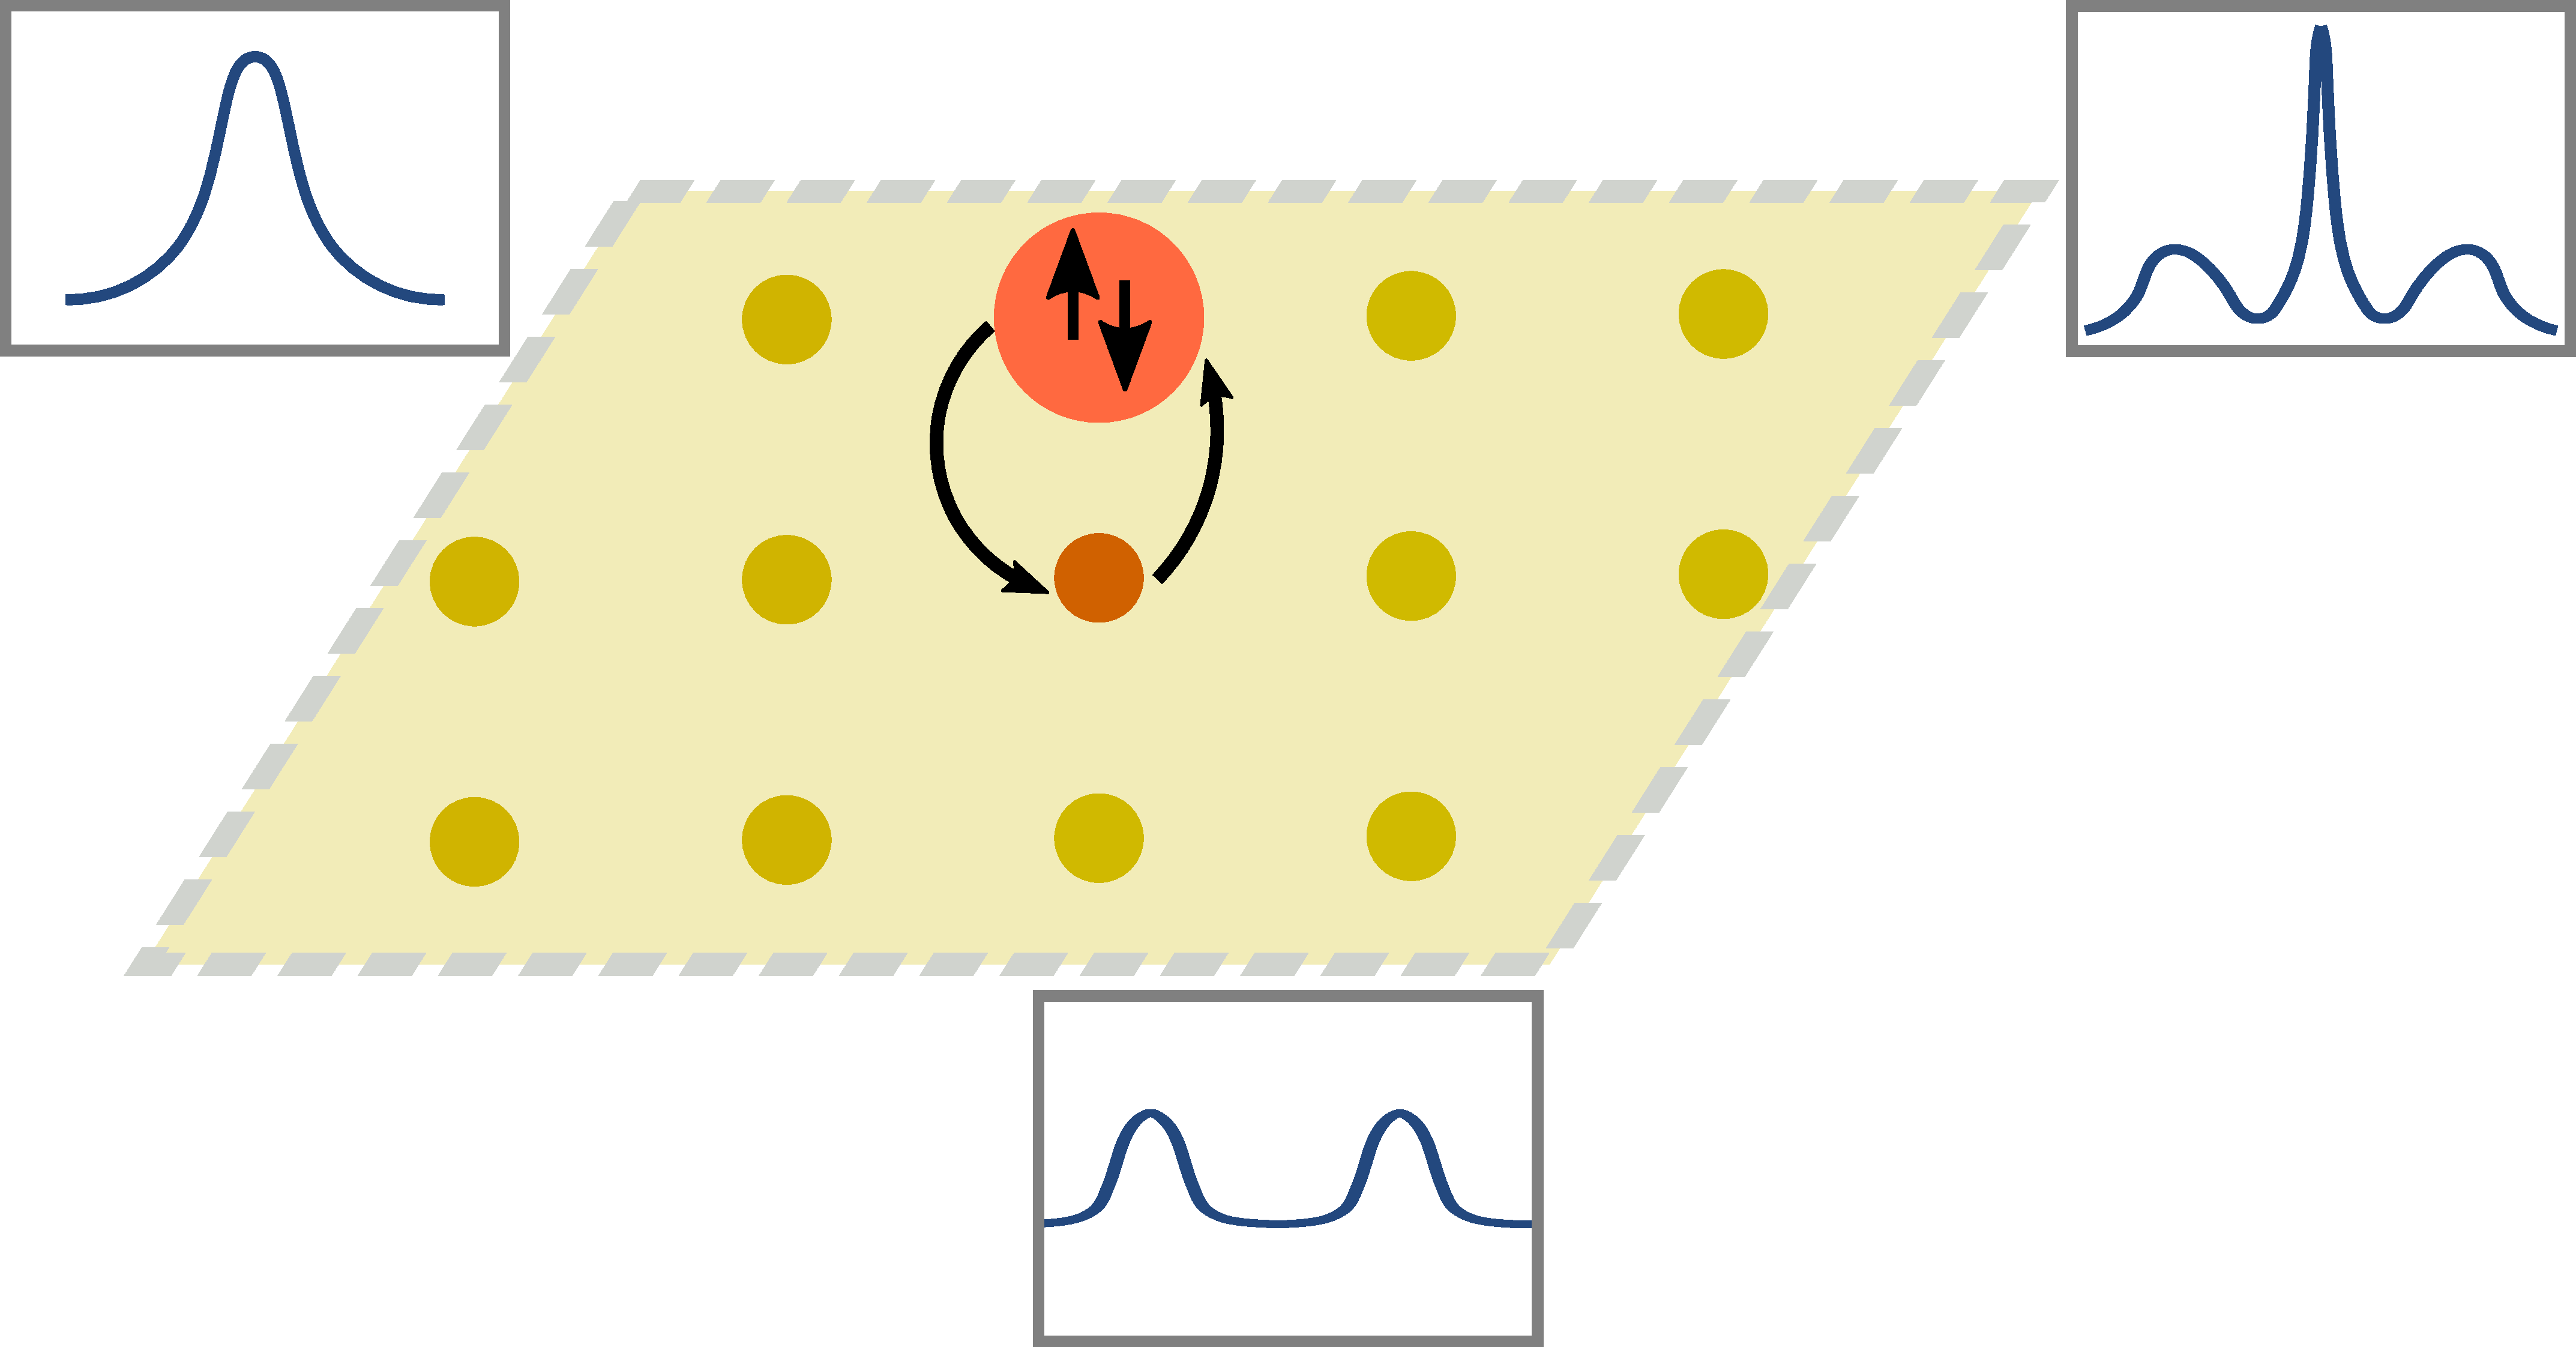
\includegraphics[width=0.4\textwidth]{figures/DMFT.pdf}

\vspace*{\fill}

\begin{itemize}
\item DMFT implementations use impurity models, exact in $d=\infty$\\[10pt]
\item Appropriate impurity model obtained through \focus{self-consistent} equations\\[10pt]
\item Displays \focus{metal-insulator transition} in Hubb. model at \(\frac{1}{2}-\)filling
\end{itemize}

\footcite*{metzner_volhardt_1989,georges_kotliar_1992,hubbard1963electron,Mott_1949}
\end{frame}

\section{Brief Summary of Results}
\begin{frame}{Brief Summary of Results}
\begin{itemize}
	\item Competition between Kondo interaction and local attractive interaction leads to \focus{multiple phases}.\\[10pt]
	\item Ground state interpolates between singlet and local moment, passing through \focus{spin+charge correlated} state.\\[10pt]
	\item Spectral function has 3-peak structure near critical point, develops gap beyond.\\[10pt]
	\item Many-particle \focus{entanglement} acts as an order parameter for the transition.
\end{itemize}
\end{frame}

\section{Extending the Anderson impurity model}
\label{the-model}
\begin{frame}{\insertsectionhead}

\[H = \overbrace{\sum_{k\sigma}\epsilon_k \tau_{k\sigma} + V \sum_{k\sigma}\left(c^\dagger_{d\sigma}c_{k\sigma} + \text{h.c.}\right)  - \frac{1}{2}U \left(\hat n_{d \uparrow} - \hat n_{d \downarrow}\right)^2}^\text{\normalsize p-h symmetric Anderson impurity model} + \underbrace{J \vec{S}_d\cdot\vec{S}_0 - U_b \left(\hat n_{0 \uparrow} - \hat n_{0 \downarrow}\right)^2}_\text{\normalsize additional terms}\]

\vspace*{\fill}

\hspace*{-30pt}
\begin{minipage}{0.55\textwidth}
\begin{itemize}
	\item \focus{spin-exchange} \(J\) between impurity-bath\\[10pt]
	\item \focus{correlation} \(U_b\) on zeroth site of bath\\[10pt]
	\item p-h symmetry is maintained\\[10pt]
	\item \(J,U_b\) \focus{compete} 
\end{itemize}
\end{minipage}
\begin{minipage}{0.5\textwidth}
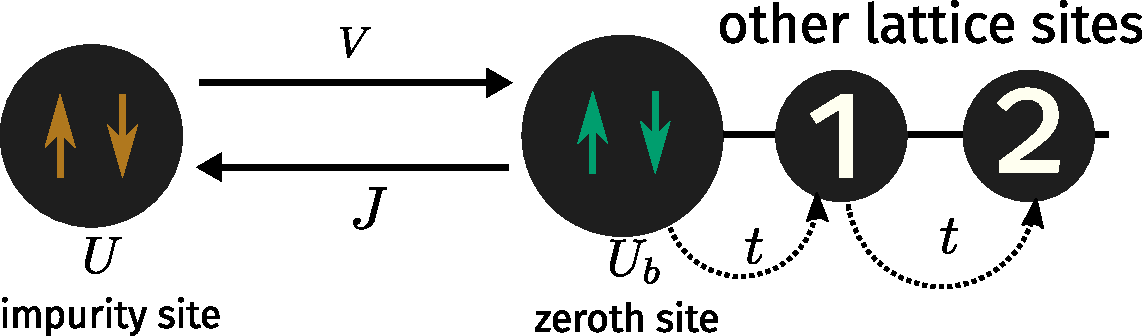
\includegraphics[width=0.99\textwidth]{figures/zeromode_bare.pdf}
\[ r \equiv -U_b/J \]
\end{minipage}

\vspace*{\fill}

\end{frame}

\section{The Unitary RG Method}
\label{method}

\begin{frame}{The Unitary RG Method: Select a UV-IR Scheme}

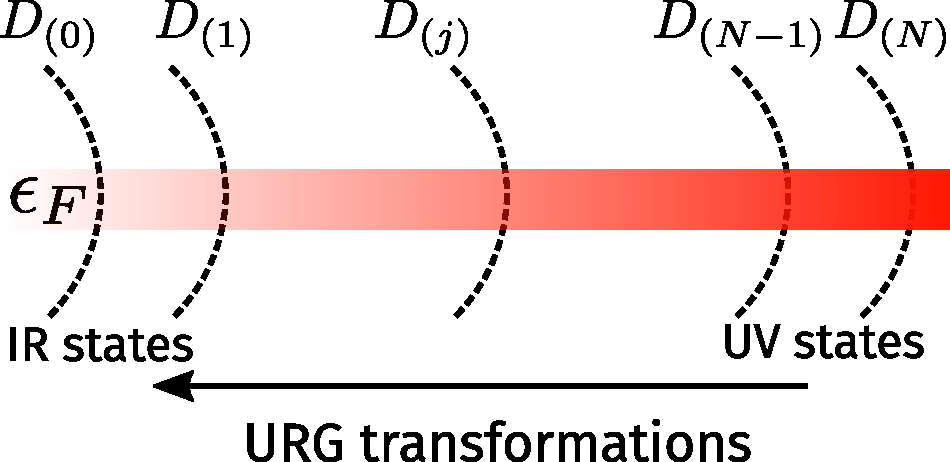
\includegraphics[width=0.6\textwidth]{figures/urg-scheme.pdf}

\vspace*{\fill}
{\Large \( j^\text{th} \text{ RG step } \longrightarrow \vec k_{j\sigma}\)}

\footcite{anirbanurg1,anirbanurg2}

\end{frame}

\begin{frame}{The Unitary RG Method: Write Hamiltonian in the basis of \(\vec k_j\)}

\vspace*{\fill}

\begin{minipage}{0.4\textwidth}
\[H_{(j)} = H_1 \hat n_j + H_0 \left(1 - \hat n_j\right) + c^\dagger_j T + T^\dagger c_j\]

\vspace*{\fill}

\[
{2^{j-1} \text{-dim.}} \longrightarrow \begin{cases}
H_1, H_0 \longrightarrow \text{diagonal parts}\\
T \longrightarrow \text{off-diagonal part}
\end{cases}
\]

\vspace*{\fill}

\[ (j) : j^\text{th} \text{ RG step}\]
\end{minipage}
\hspace*{\fill}
\begin{minipage}{0.5\textwidth}
\begin{figure}
	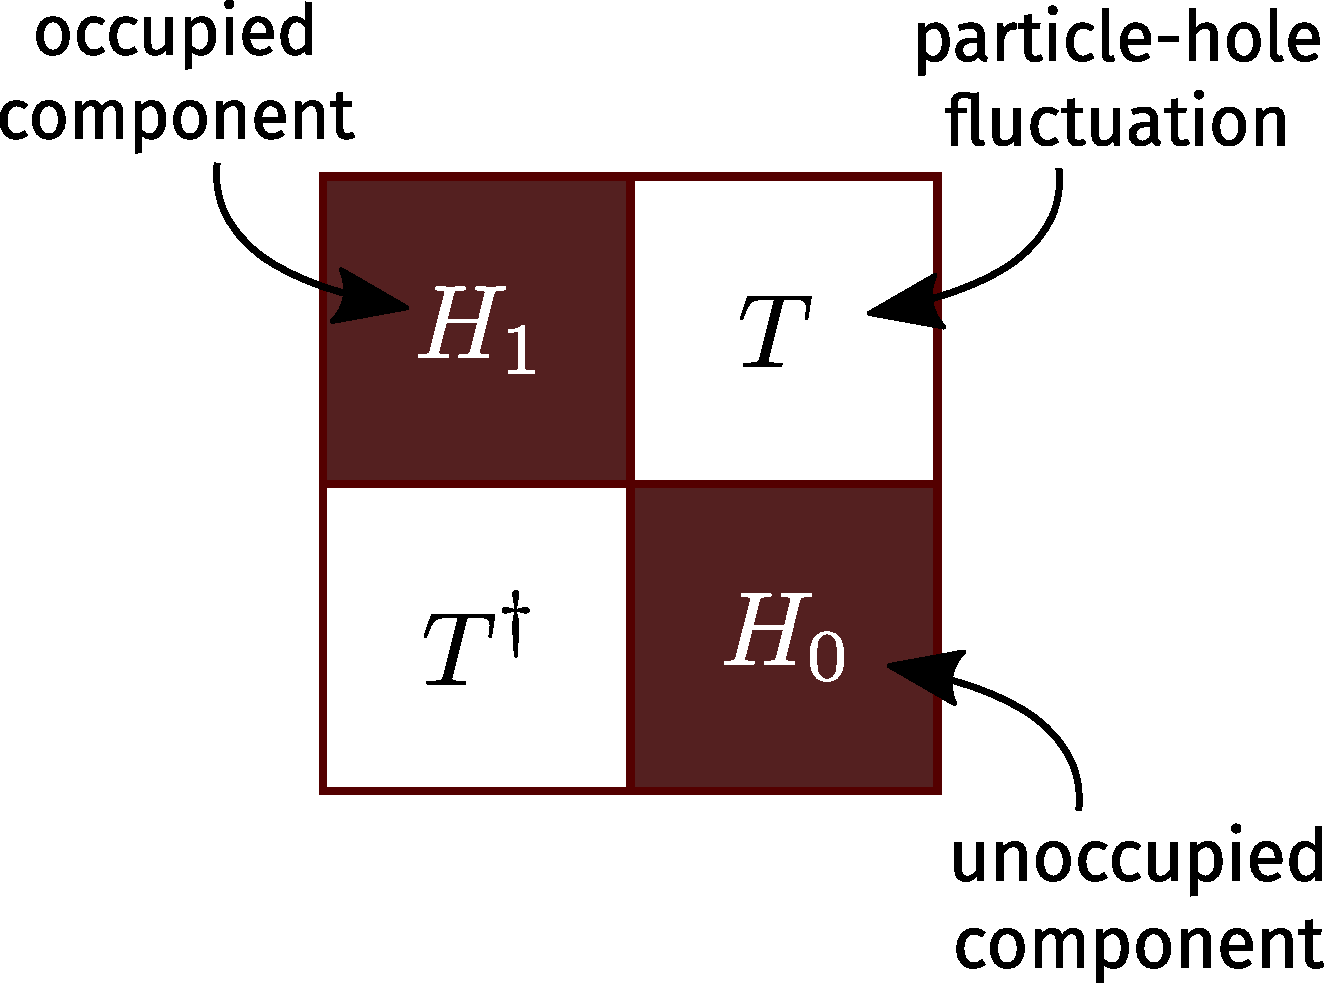
\includegraphics[width=0.9\textwidth]{figures/urg_ham.pdf}
\end{figure}
\end{minipage}

\vspace*{\fill}

\footcite{anirbanurg1,anirbanurg2}
\end{frame}

\begin{frame}{The Unitary RG Method: Rotate and kill off-diagonal blocks}

\vspace*{\fill}

\begin{minipage}{0.5\textwidth}
\centering
\(H_{(j-1)} = U_{(j)} H_{(j)} U_{(j)}^\dagger\)\\[20pt]
\(U_{(j)} = \frac{1}{\sqrt 2}\left(1 - \eta_{(j)} + \eta_{(j)}^\dagger\right)\)\\[20pt]
many-particle rotation of Hamiltonian
\vspace*{\fill}
\end{minipage}
\hspace*{\fill}
\begin{minipage}{0.45\textwidth}
\begin{figure}
	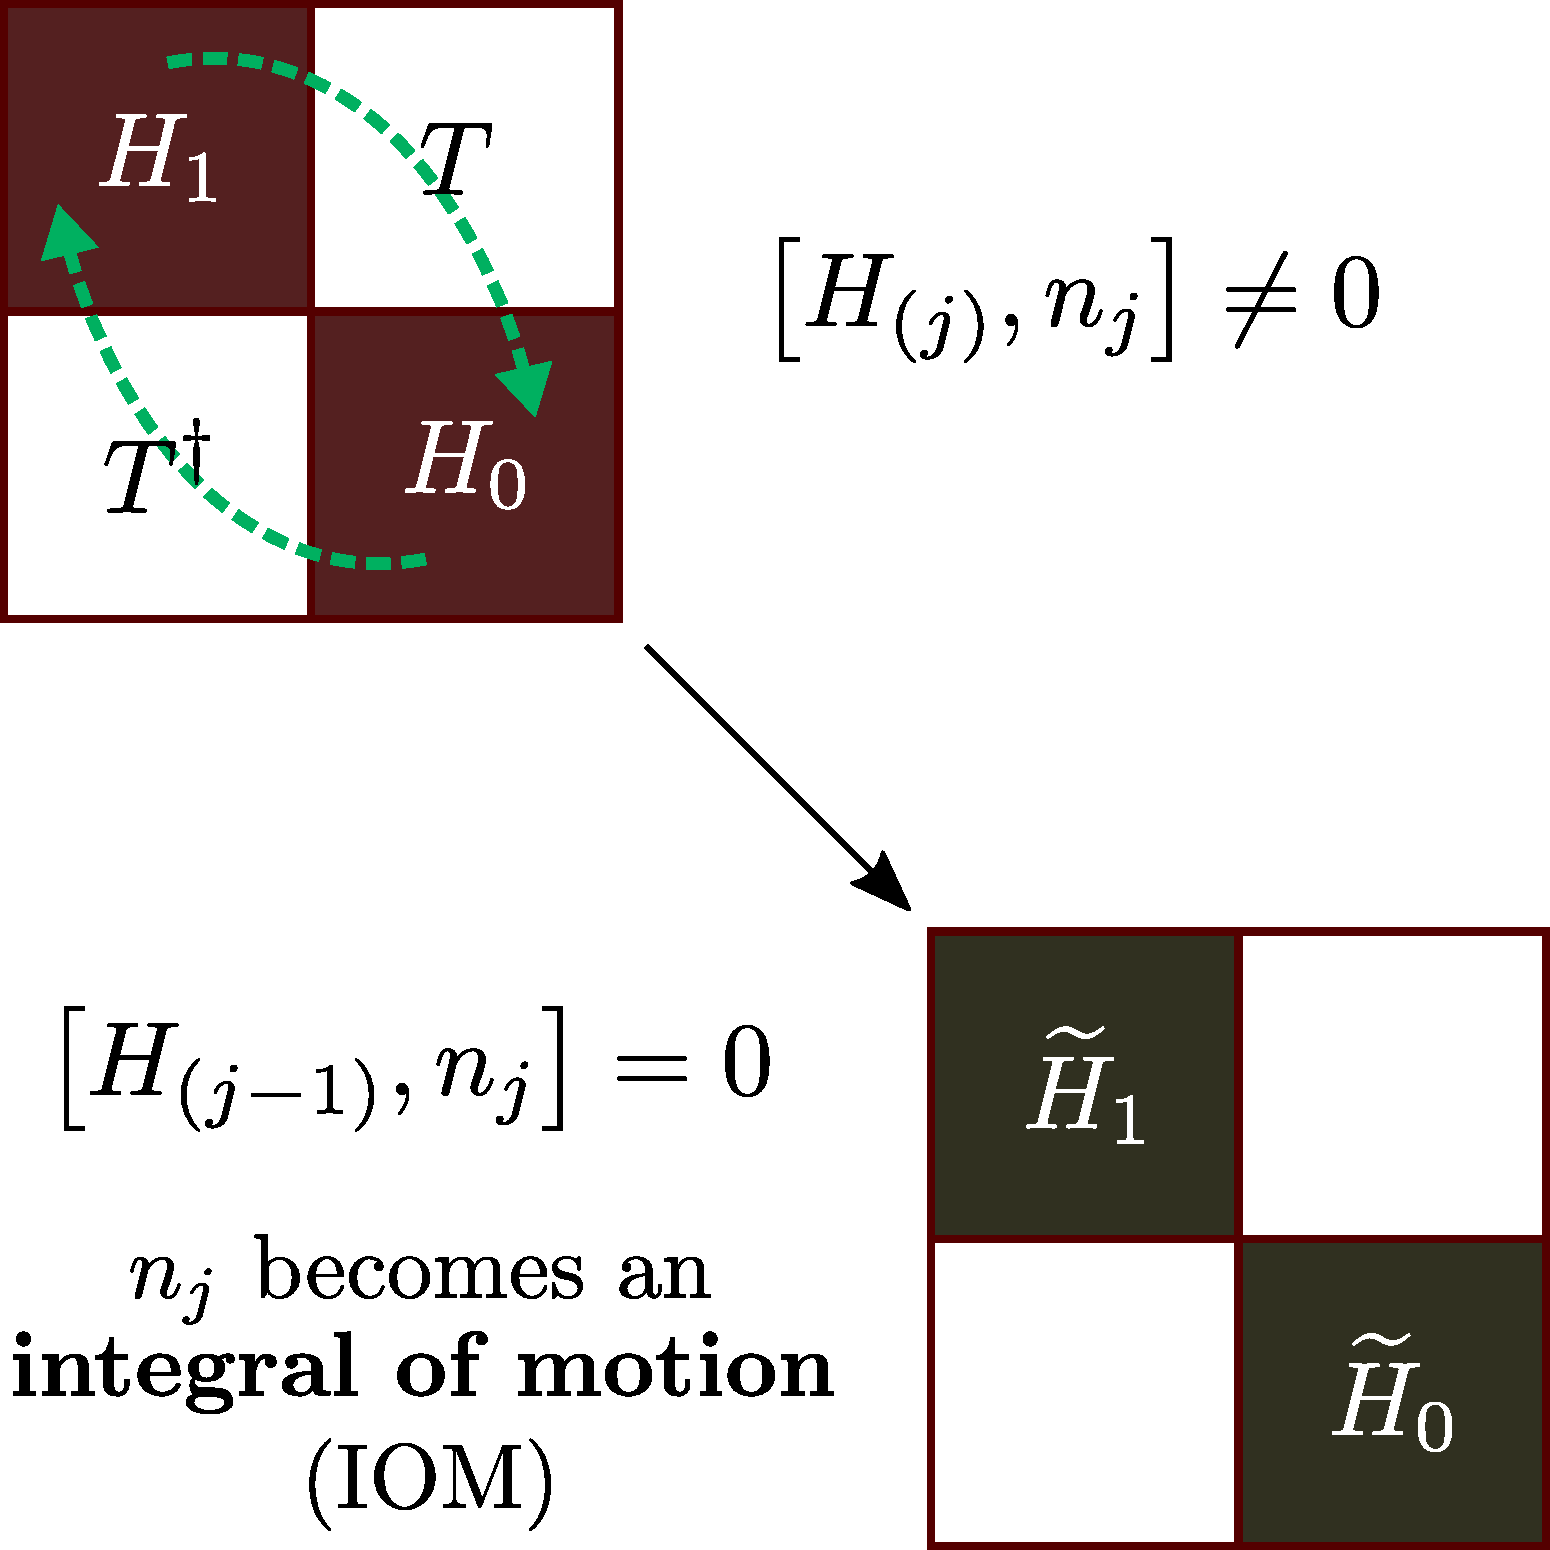
\includegraphics[width=0.8\textwidth]{figures/urg_rot.pdf}
\end{figure}
\end{minipage}

\footcite{anirbanurg1,anirbanurg2}
\end{frame}

\begin{frame}{The Unitary RG Method: Rotate and kill off-diagonal blocks}

\vspace*{\fill}

\begin{minipage}{0.5\textwidth}
\centering
\focus{Fermionic}: \(\left\{\eta_{(j)}, \eta^\dagger_{(j)}\right\} = 1 \)\\[20pt]
\( \eta^\dagger_{(j)} = \frac{1}{\hat \omega_{(j)} - H_D}c^\dagger_j T \Bigg \} \rightarrow {\text{many-particle}\atop{\text{rotation}}}\)\\[20pt]
\(\hat \omega\)~: \focus{quantum fluctuation} operator
\vspace*{\fill}
\end{minipage}
\hspace*{\fill}
\begin{minipage}{0.45\textwidth}
\begin{figure}
	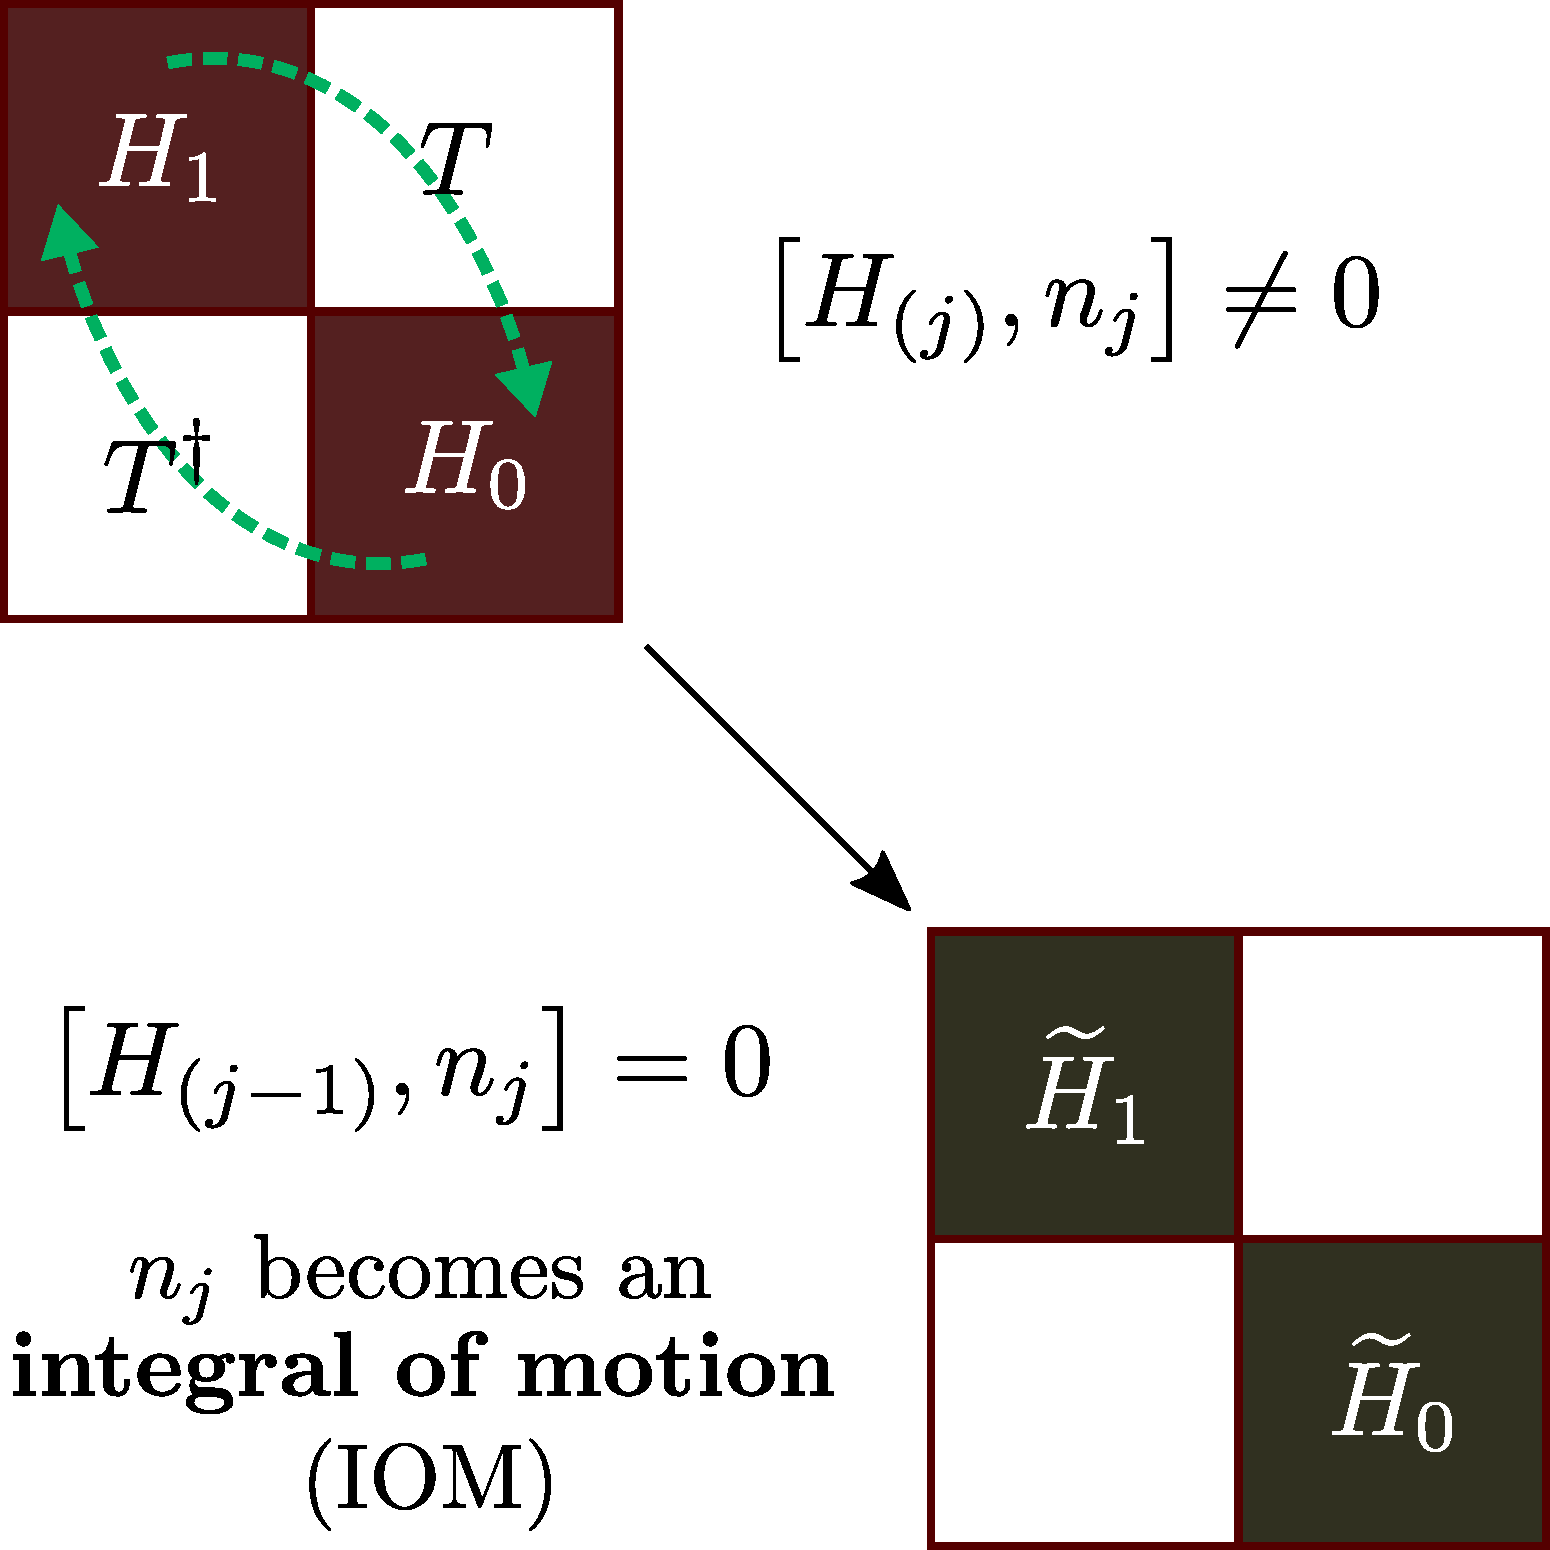
\includegraphics[width=0.8\textwidth]{figures/urg_rot.pdf}
\end{figure}
\end{minipage}

\footcite{anirbanurg1,anirbanurg2}
\end{frame}

\begin{frame}{The Unitary RG Method: Repeat with new Hamiltonian}

\begin{minipage}{0.53\textwidth}
	\[H_{(j-1)} = \widetilde H_1 \hat n_j + \widetilde H_0 \left(1 - \hat n_j\right)\]
	\[\widetilde H_1 = H_1 \hat n_{j-1} + H_0 \left(1 - \hat n_{j-1}\right) + c^\dagger_{j-1} T + T^\dagger c_{j-1}\]
\vspace*{\fill}
\end{minipage}
\hspace*{\fill}
\begin{minipage}{0.45\textwidth}
\begin{figure}
	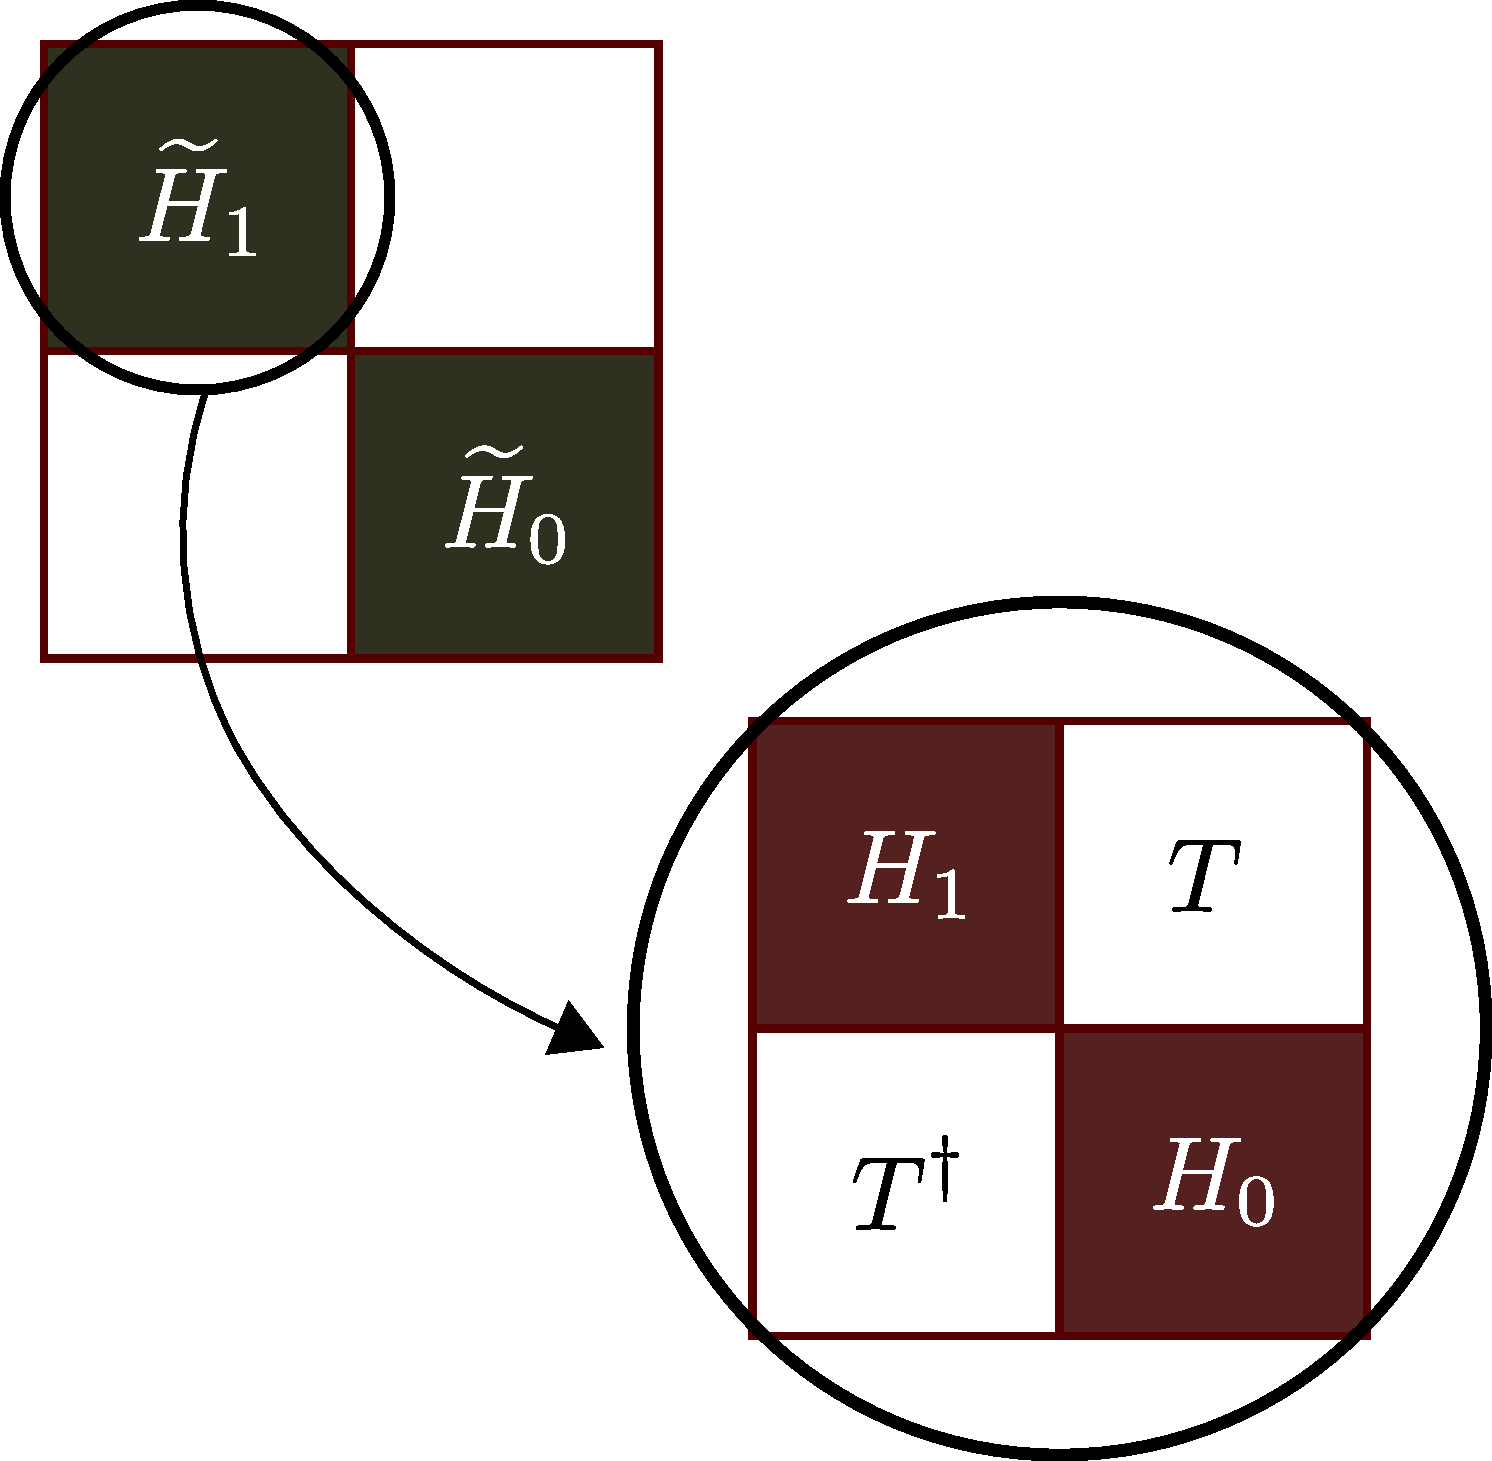
\includegraphics[width=\textwidth]{figures/urg_next.pdf}
\end{figure}
\end{minipage}

\footcite{anirbanurg1,anirbanurg2}
\end{frame}

\begin{frame}{The Unitary RG Method: RG Equations and Fixed Point}

\begin{minipage}{0.55\textwidth}
\centering
\(\Delta H_{(j)} = \left(\hat n_j - \frac{1}{2}\right) \left\{c^\dagger_j T, \eta_{(j)}\right\}\)\\[20pt]
\(\eta^\dagger_{(j)} = \frac{1}{\hat \omega_{(j)} - H_D}c^\dagger_j T\) \\[20pt]
\(\text{{Fixed point:}}~ ~ ~\hat \omega_{(j^*)} - \left(H_D\right)^* = 0\)\\[20pt]
\focus{eigenvalue of \(\hat \omega\) coincides with that of \(H\)}

\end{minipage}
\hspace*{\fill}
\begin{minipage}{0.4\textwidth}
	\centering
	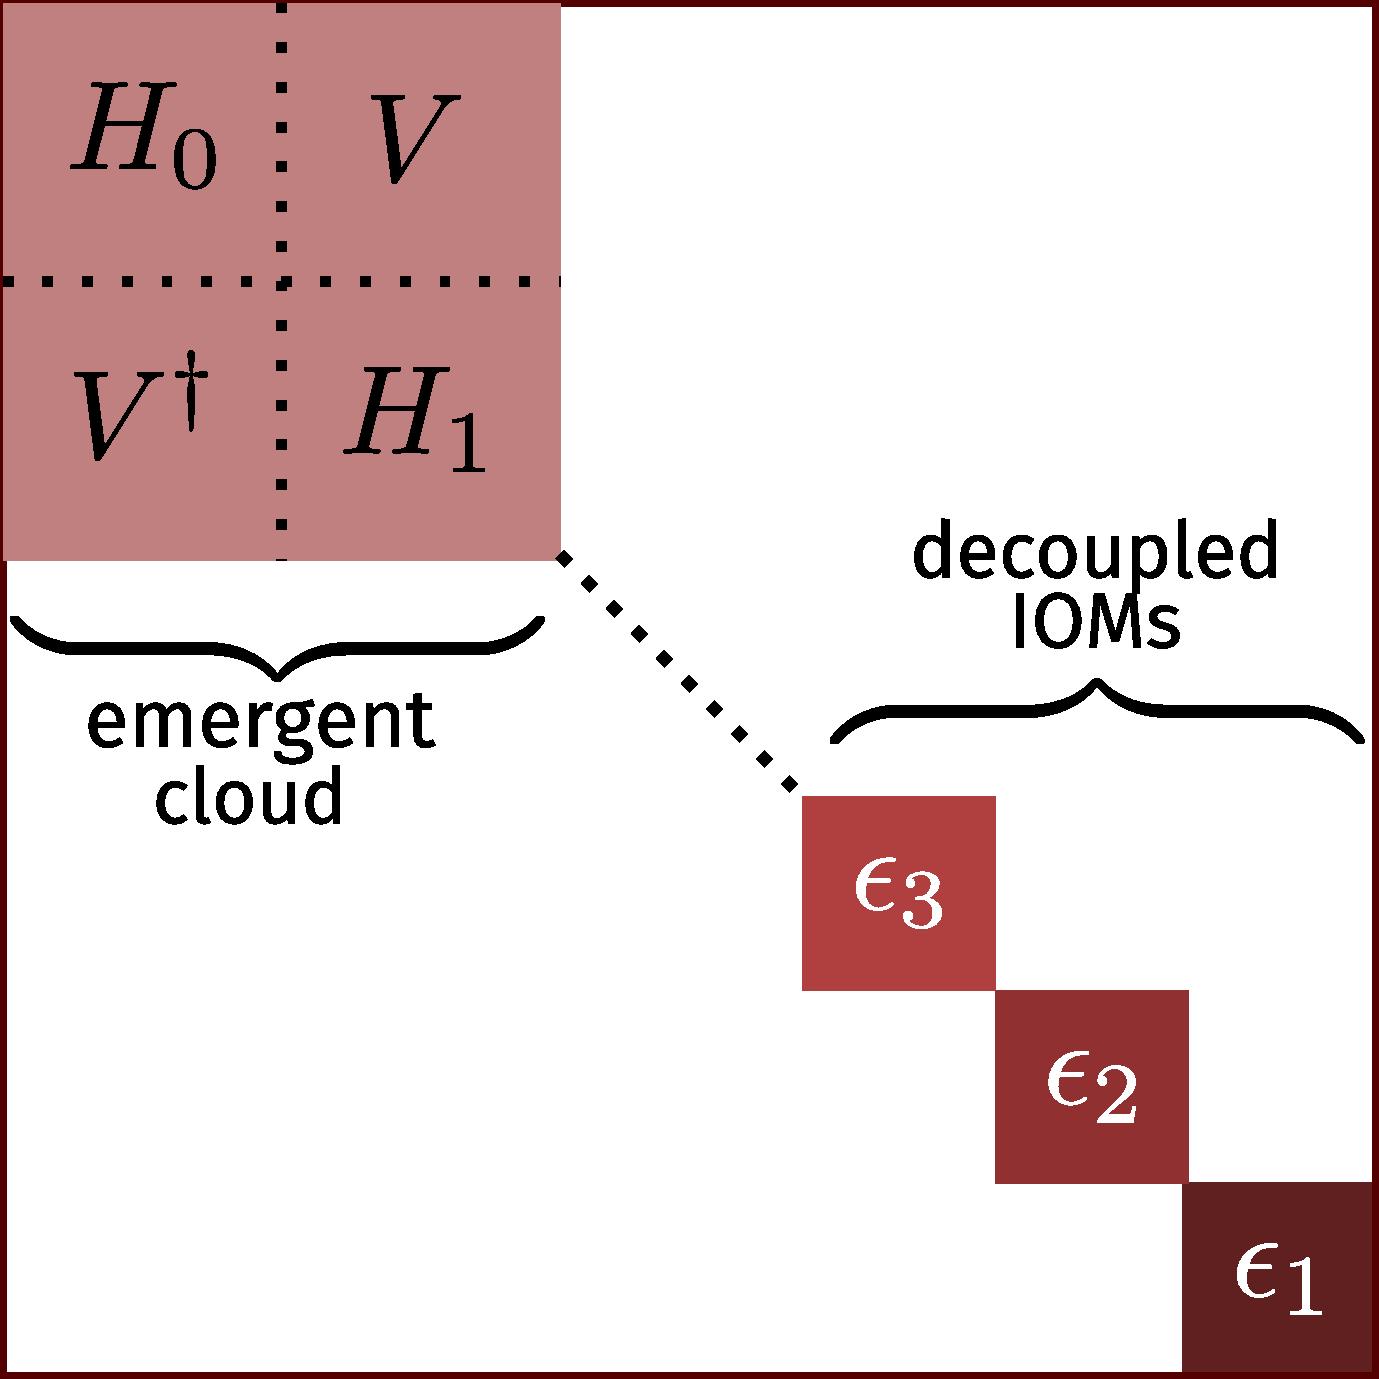
\includegraphics[width=0.9\textwidth]{figures/urg_ham_full.pdf}
\end{minipage}
\vspace*{\fill}

\footcite{anirbanurg1,anirbanurg2}
\end{frame}

\begin{frame}{The Unitary RG Method: Novel Features of the Method}

\vspace*{\fill}
\begin{itemize}
	\item \focus{Quantum fluctuation scale} \(\hat \omega\)	that tracks all orders of renormalisation\\[15pt]
	\item Finite-valued fixed points for finite systems - leads to \focus{emergent DOFs}\\[15pt]
	\item \focus{Spectrum-preserving} unitary transformations - partition function left unchanged\\[15pt]
	\item Tractable low-energy effective Hamiltonians - allows \focus{renormalised perturbation theory} 
\end{itemize}
\vspace*{\fill}

\footcite{santanukagome,anirbanmott1,anirbanmott2,anirban_mott_ent,1dhubjhep,siddharthacpi,anirban_kondo}
\end{frame}

\section{RG Flows \& Phase Diagram}
\begin{frame}{Coupling RG Flows}
\begin{itemize}
\item \(U_b\) is marginal\\[10pt]
\item For \(-U_b < J/4\): \(J,V\) are relevant, \(U\) is irrelevant\\[10pt]
\item For \(-U_b > J/4\): \(J,V\) are irrelevant, \(U\) is "relevant"\\[10pt]
\item \focus{Transition} at \(r = -U_b/J = 1/4\)
\end{itemize}

\vspace*{\fill}

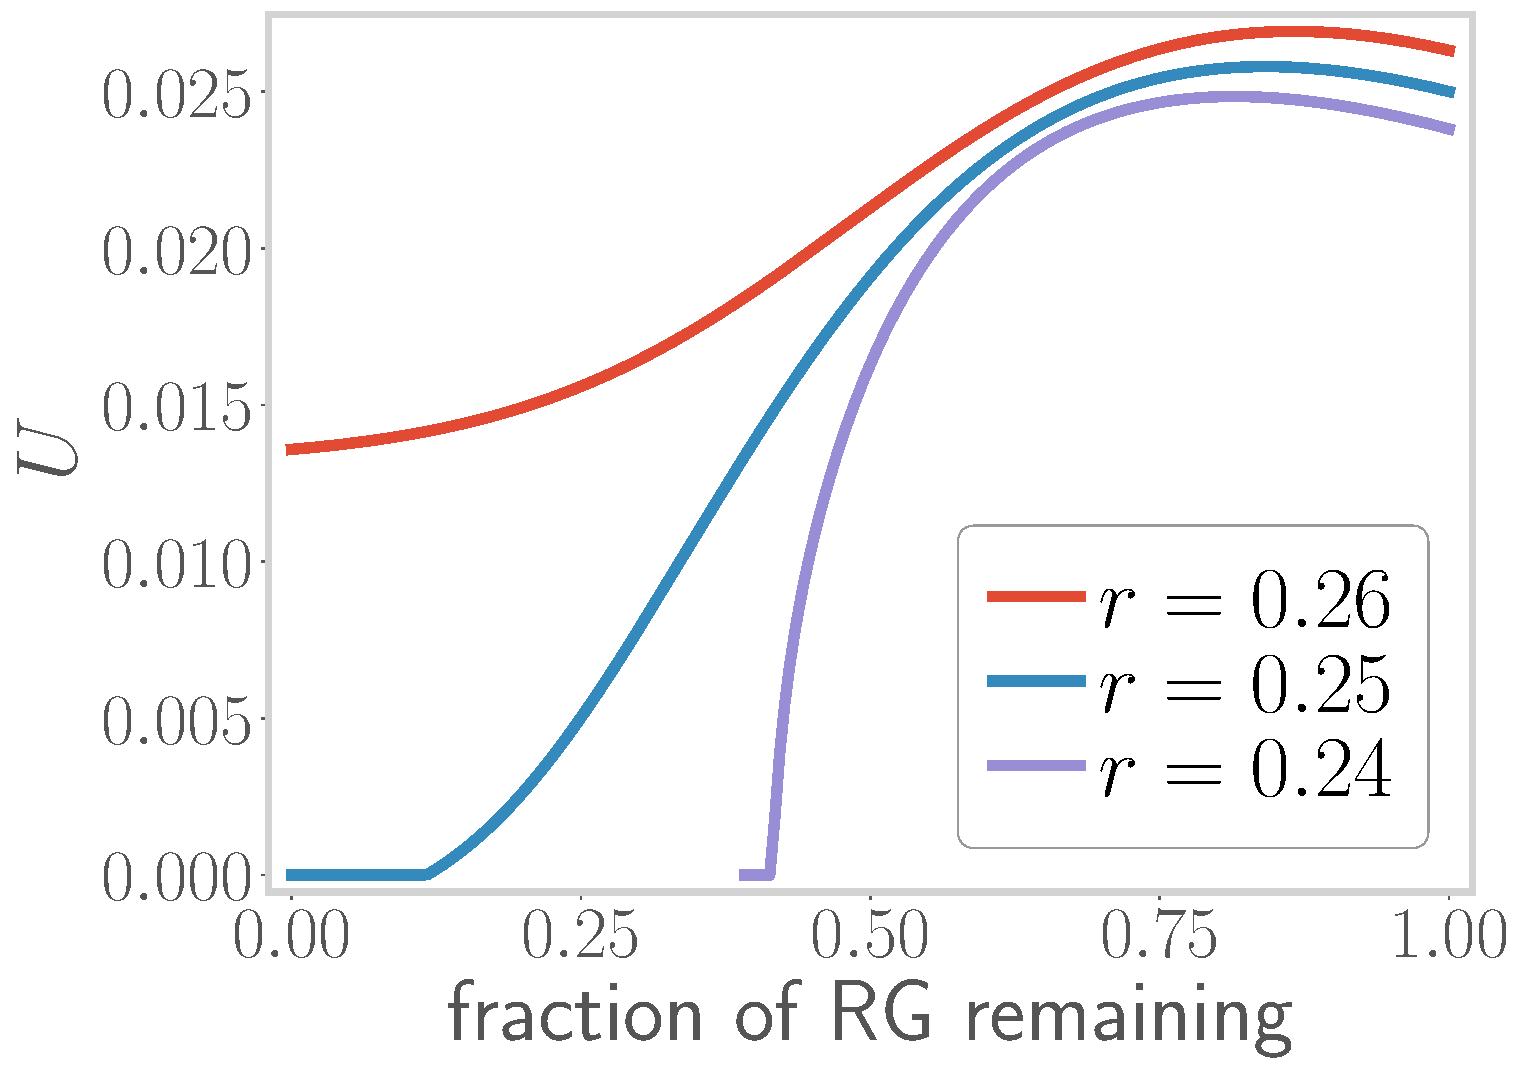
\includegraphics[width=0.32\textwidth]{figures/U_Ub.pdf}
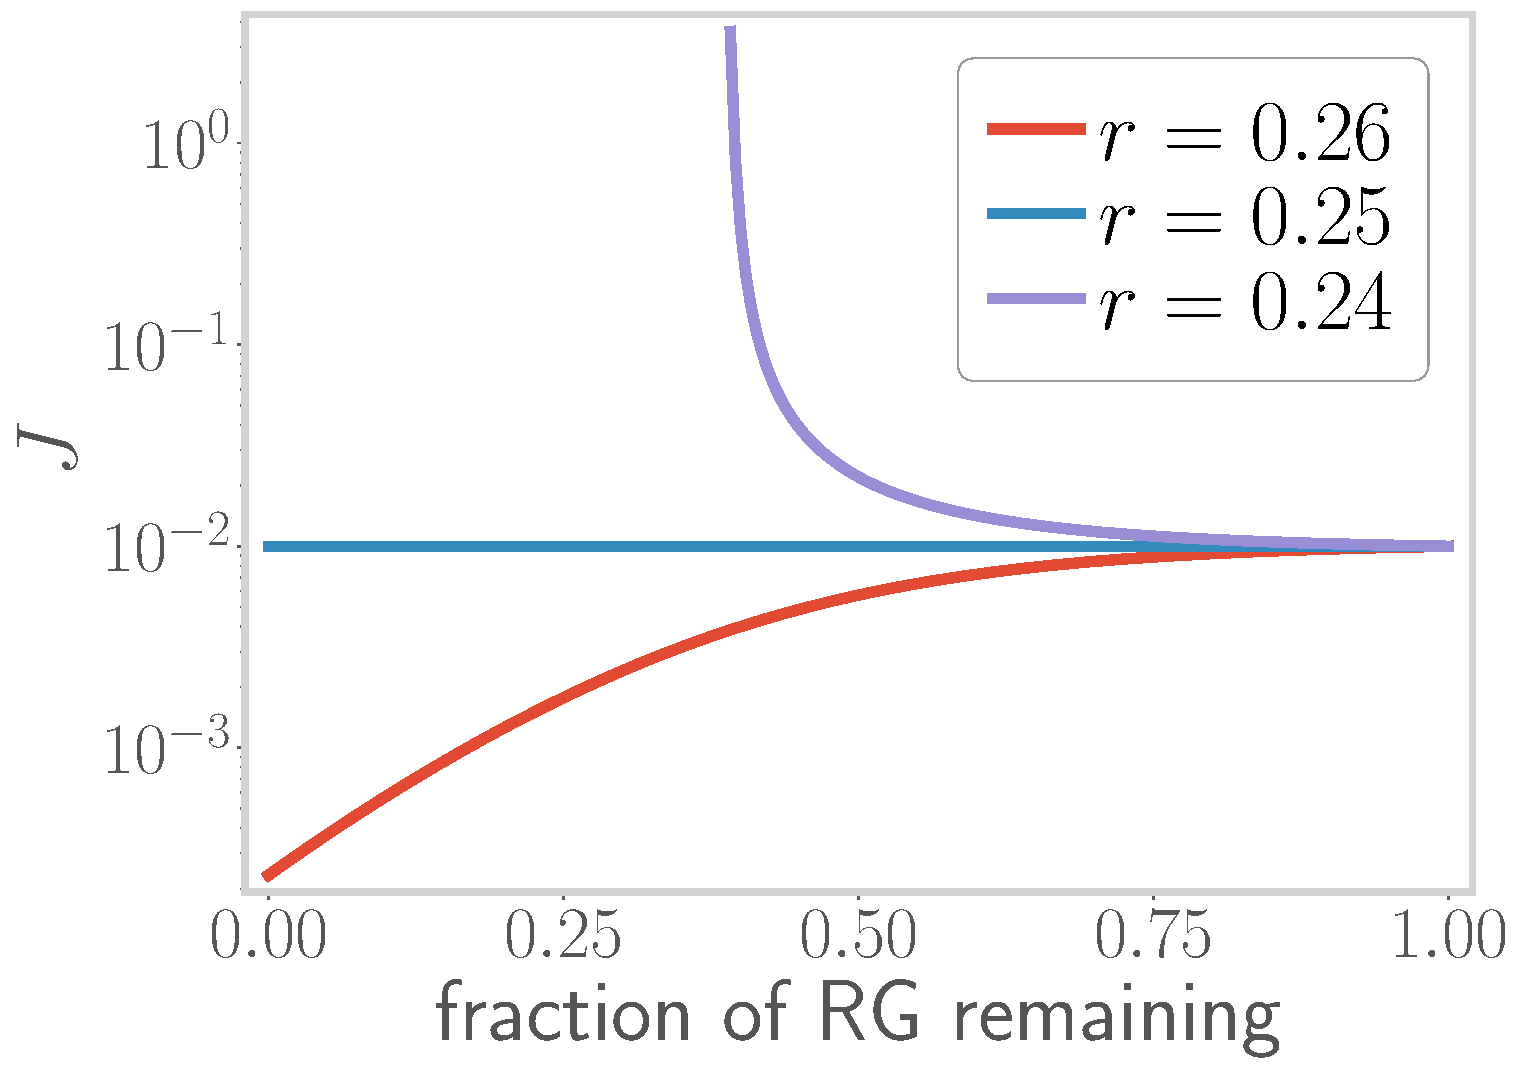
\includegraphics[width=0.32\textwidth]{figures/J_Ub.pdf}
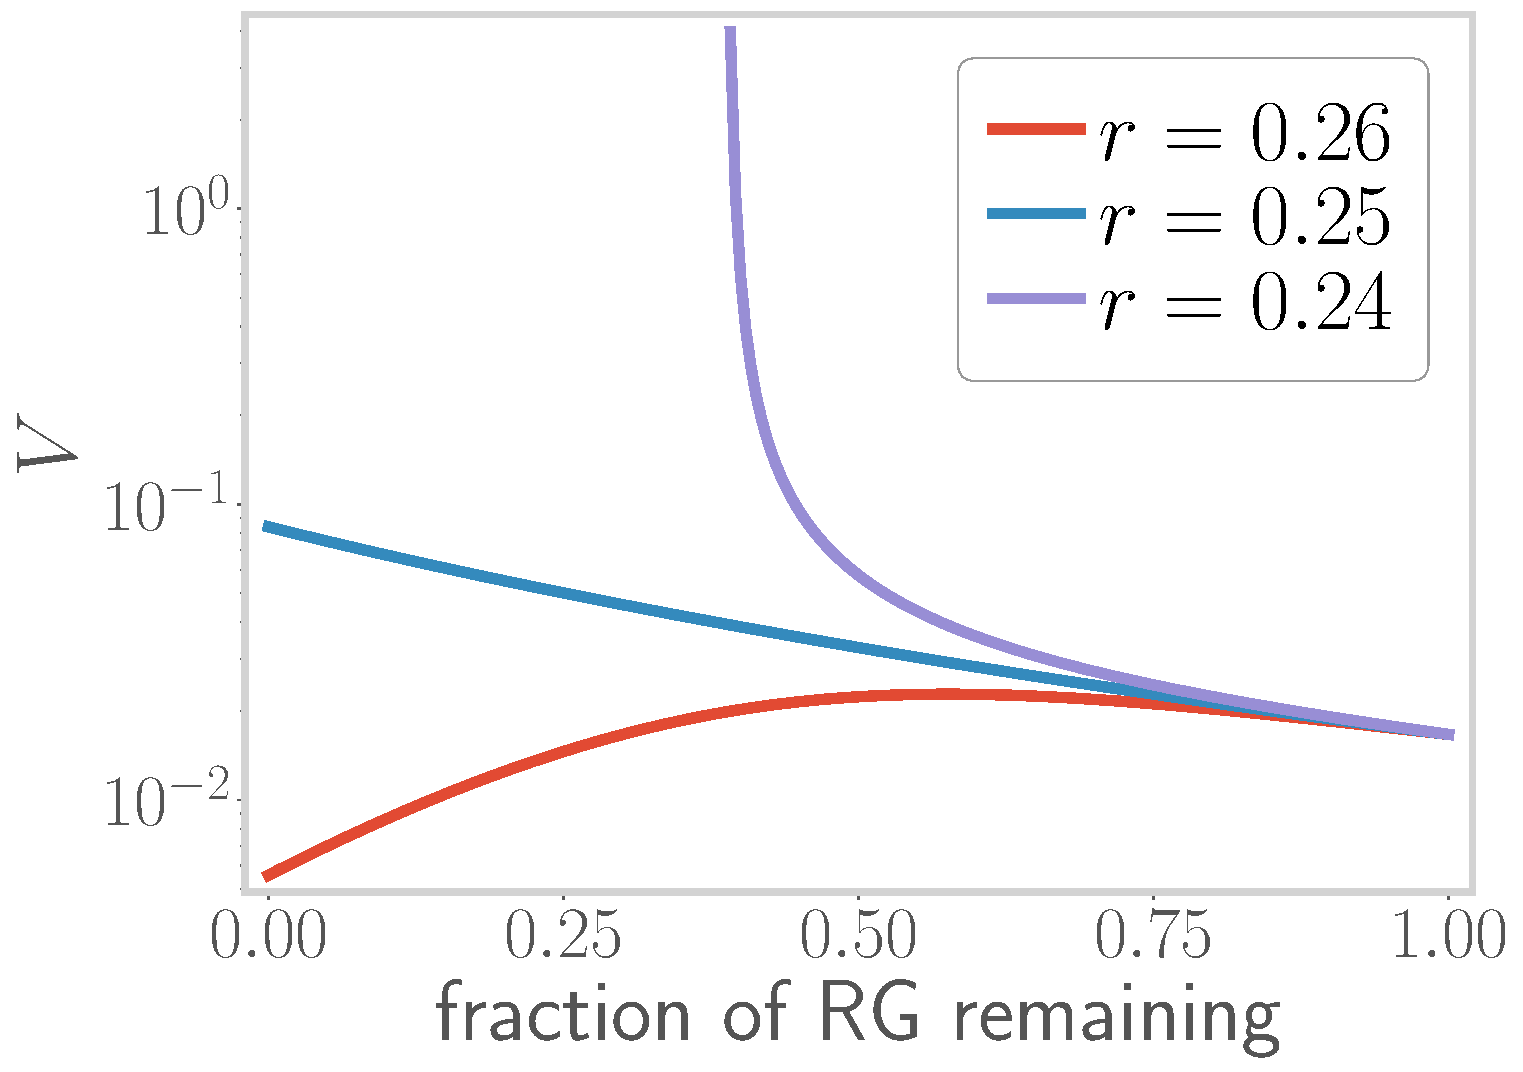
\includegraphics[width=0.32\textwidth]{figures/V_Ub.pdf}

\end{frame}

\begin{frame}{Phase diagram: \(U_b = -U/10\)}

\hspace*{-30pt}
\begin{minipage}{0.55\textwidth}
\begin{itemize}
	\item {\bf\color{orange}Red}: \(V,J\) \(\big\uparrow\), \(U\) \(\big\downarrow\): local Fl\\[10pt]
	\item {\bf\color{blue}Blue}: \(V,J\) \(\big\downarrow\), \(U\) \(\big\uparrow\): local moment
\end{itemize}
\end{minipage}
\begin{minipage}{0.5\textwidth}
\begin{itemize}
	\item {\bf\color{yellow}Yellow}: \(V,U\) survive: spin+charge\\[10pt]
	\item {\bf\color{gray}Grey}: \(U,V,J\) all \(\big\downarrow\)
\end{itemize}
\end{minipage}

\vspace*{\fill}

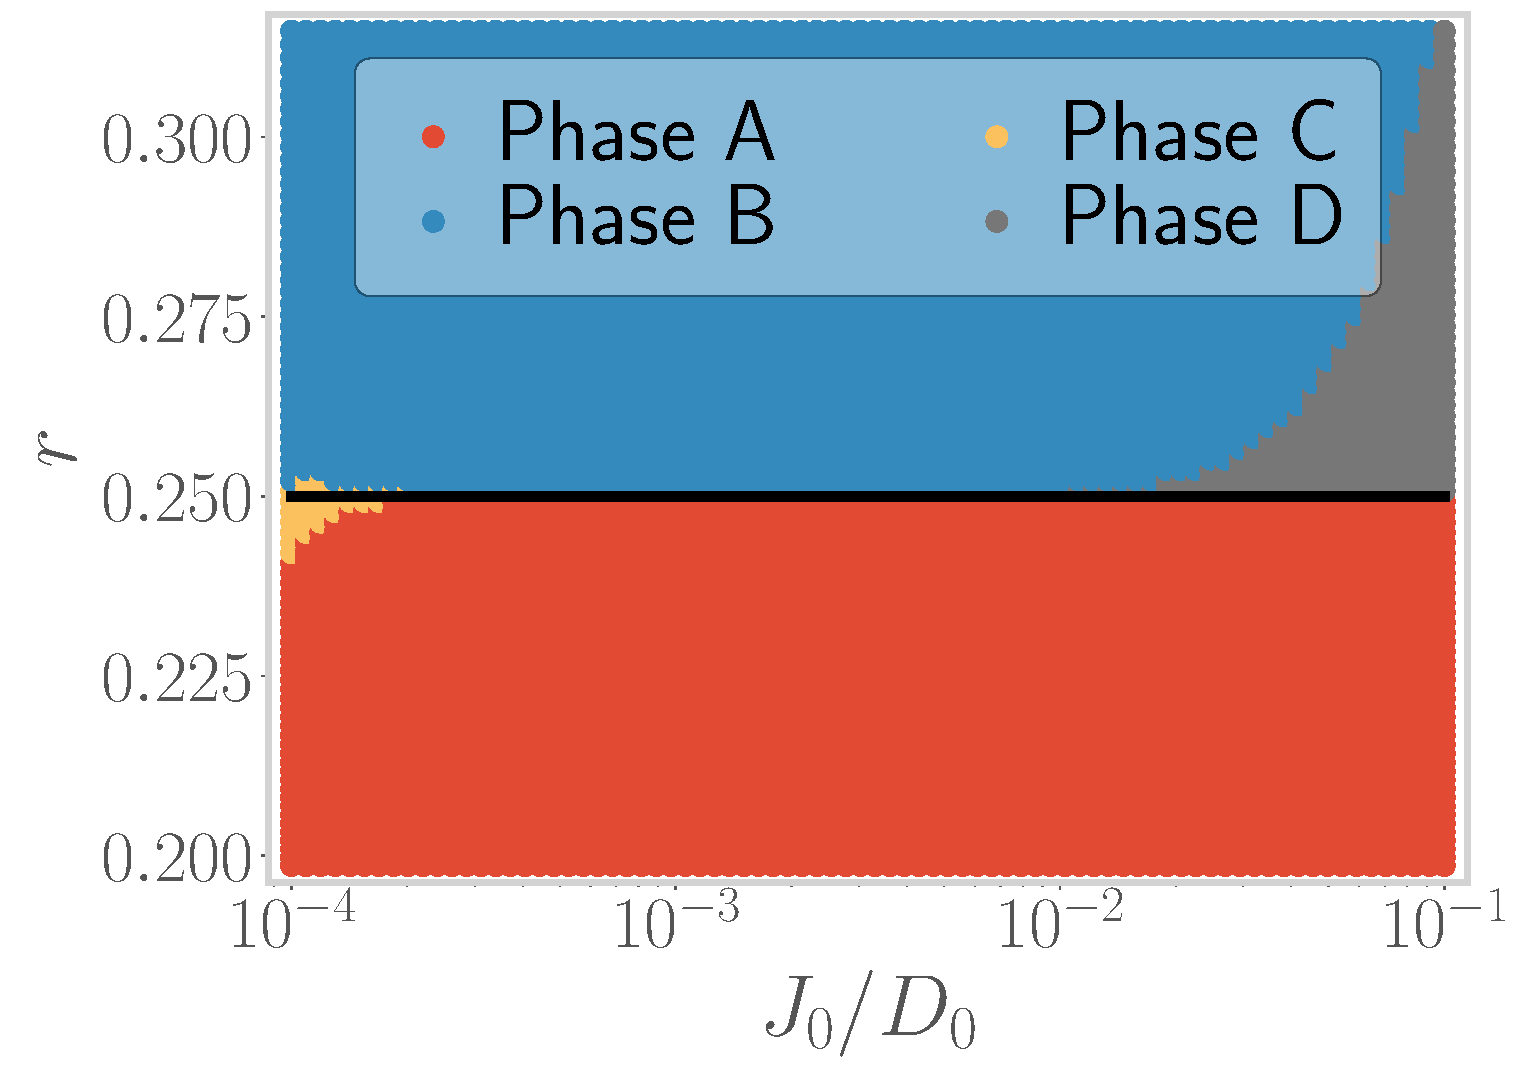
\includegraphics[width=0.5\textwidth]{figures/phase-map-MIT.pdf}
\end{frame}

\begin{frame}{Growth of charge isospin fluctuations}
\begin{minipage}{0.5\textwidth}
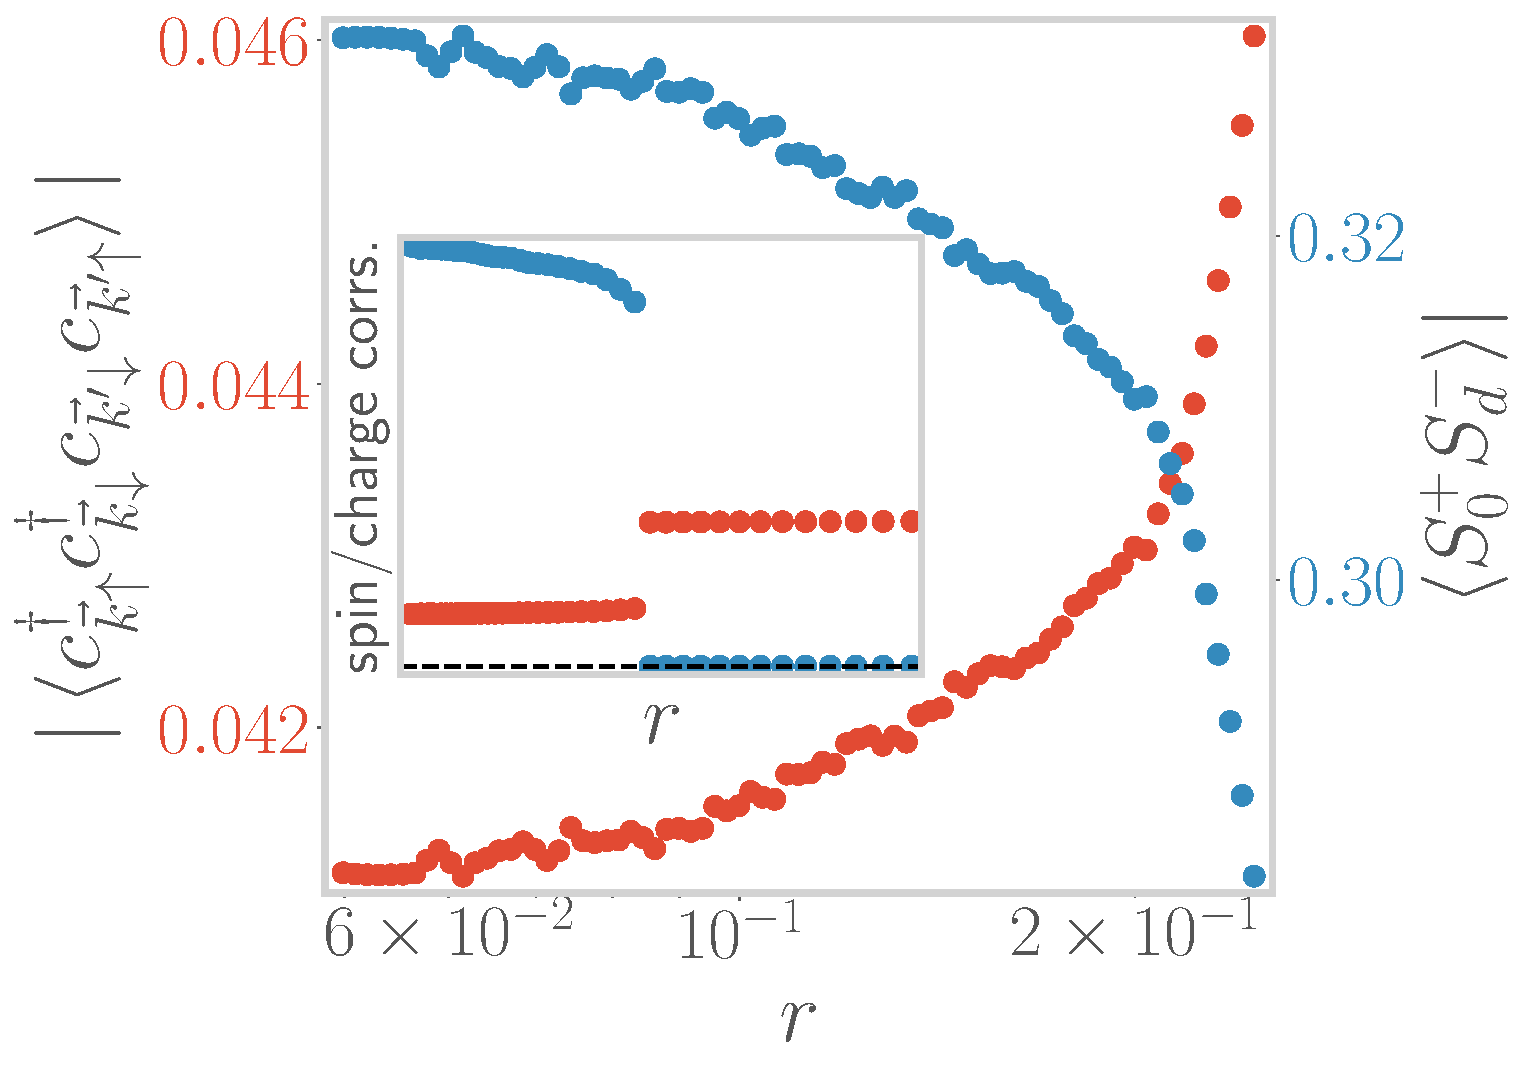
\includegraphics[width=\textwidth]{figures/odlro.pdf}
\end{minipage}
\begin{minipage}{0.49\textwidth}
\begin{itemize}
\item Impurity is no longer screened\\[10pt]
\item \(S_d^\pm S_0^\mp\) replaced by isospin flucts.\\[10pt]
\item Arises from \(U_b\) term
\end{itemize}
\end{minipage}
\end{frame}

\section{Low-energy effective Hamiltonian and the ground state}

\begin{frame}{Fixed-point Hamiltonian}
	\[ \mathcal{H}^* = -\frac{1}{2}U^*\left(\hat n_{d \uparrow} - \hat n_{d \downarrow}\right)^2 + \sum_{\sigma,\vec k:|\epsilon_{\vec k}| < D^*} \epsilon_{\vec k} \tau_{\vec k,\sigma} - U_b^* \hat n_{0 \uparrow} \hat n_{0 \downarrow} + V^*\sum_\sigma \left( c^\dagger_{d\sigma}c_{0\sigma} + \text{h.c.}\right) + J^* \vec{S}_d\cdot\vec{S}_0\]
	
	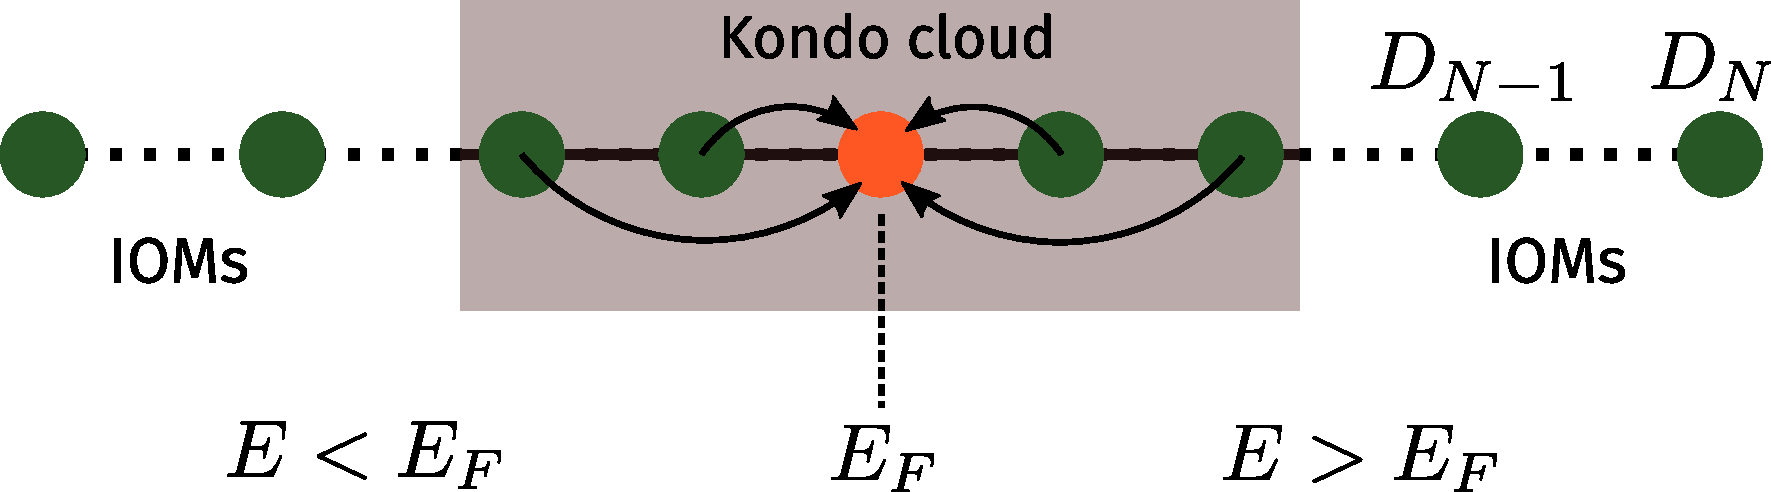
\includegraphics[width=0.6\textwidth]{figures/kondo_fp_1D.pdf}
\end{frame}

\begin{frame}{Screened regime: \(-U_b < J/4 \)}
\hspace*{-20pt}
\begin{minipage}{0.6\textwidth}
\[\mathcal{H}_\text{eff}^\text{sc} = J^* \vec{S}_d\cdot\vec{S}_0 - U_b \hat n_{0 \uparrow} \hat n_{0 \downarrow} + \sum_{\sigma,\vec k:|\epsilon_{\vec k}| < D^*} \epsilon_{\vec k} \tau_{\vec k,\sigma}\]
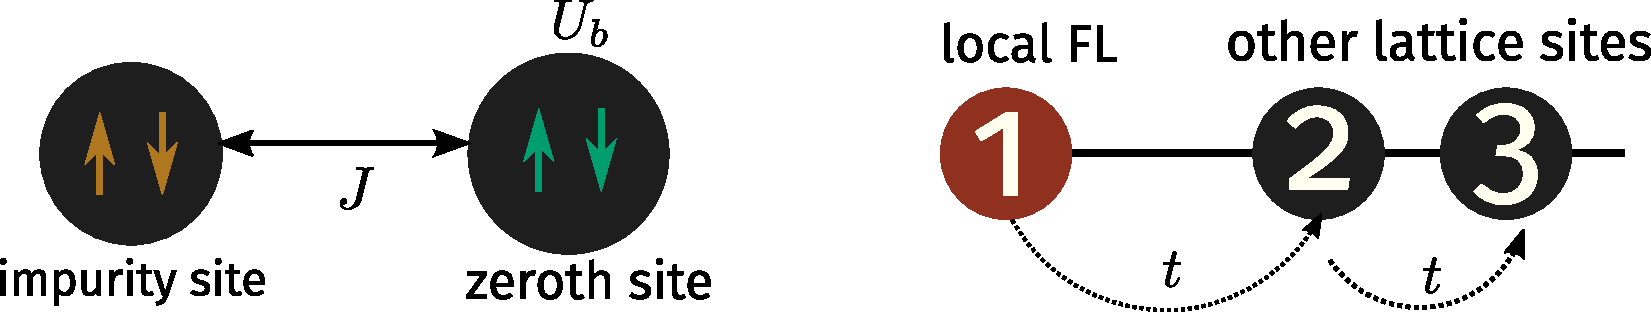
\includegraphics[width=0.99\textwidth]{figures/singlet.pdf}
\end{minipage}
\hspace*{10pt}
\begin{minipage}{0.39\textwidth}
	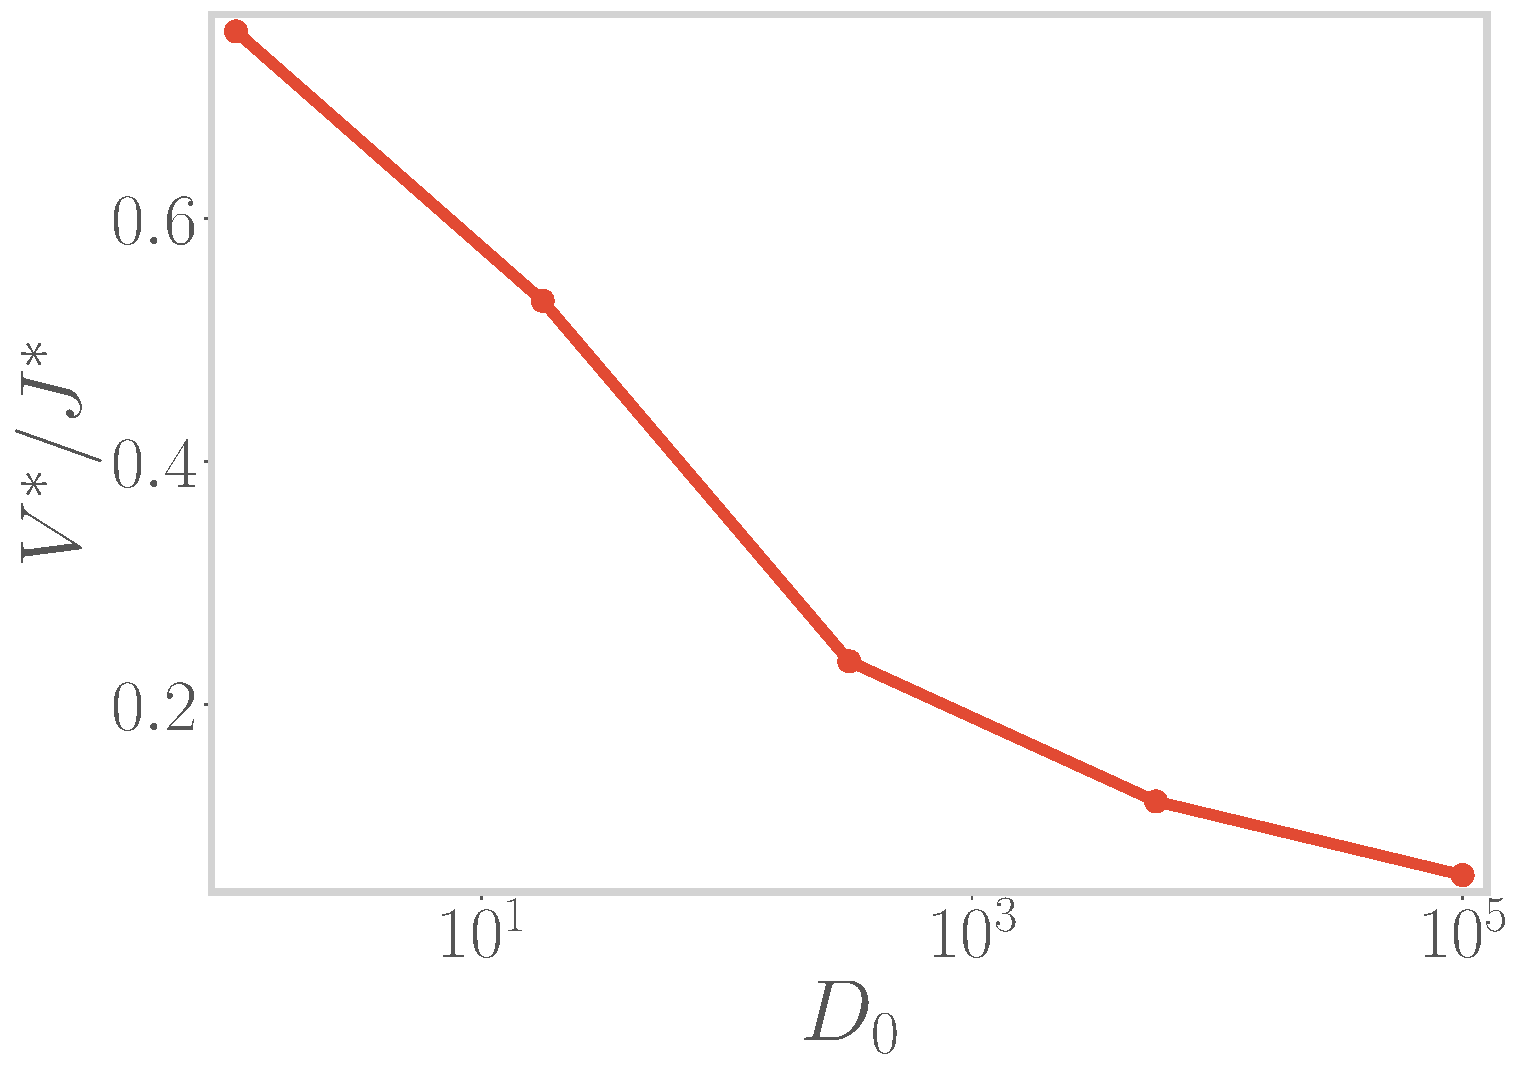
\includegraphics[width=0.99\textwidth]{figures/J_bandwidth.pdf}
\end{minipage}

\vspace*{\fill}

\focus{singlet} ground state ~ ~ ~ {\LARGE +} ~ ~ ~ \focus{local FL} excitations

\vspace*{\fill}

\footcite{wilson1975,nozieres1974fermi}
\end{frame}

\begin{frame}{Unscreened regime: \(-U_b > J/4 \)}

\[\mathcal{H}_\text{eff}^\text{uns} = -\frac{1}{2}U^*\left(\hat n_{d \uparrow} - \hat n_{d \downarrow}\right)^2 - U_b \hat n_{0 \uparrow} \hat n_{0 \downarrow} + \sum_{\sigma,\vec k:|\epsilon_{\vec k}| < D^*} \epsilon_{\vec k} \tau_{\vec k,\sigma}\]

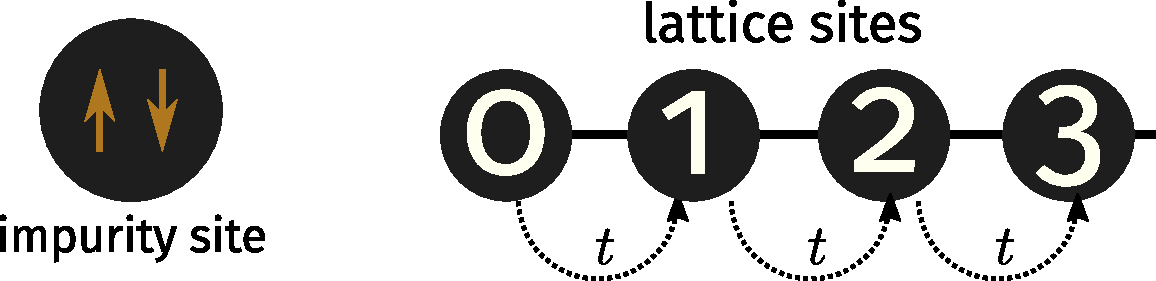
\includegraphics[width=0.6\textwidth]{figures/local-m.pdf}

\vspace*{\fill}

\focus{local moment} ground state 

\end{frame}

\begin{frame}{Near the critical point: \(-U_b = J/4 \)}

\begin{minipage}{0.5\textwidth}

\centering

Both \(V,J\) survive

\vspace*{20pt}

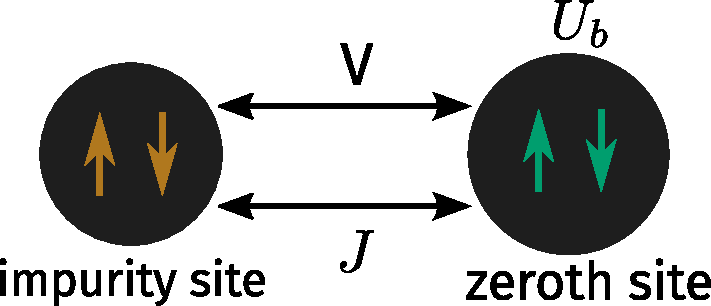
\includegraphics[width=0.8\textwidth]{figures/spin-charge.pdf}

\end{minipage}
\begin{minipage}{0.49\textwidth}
\centering
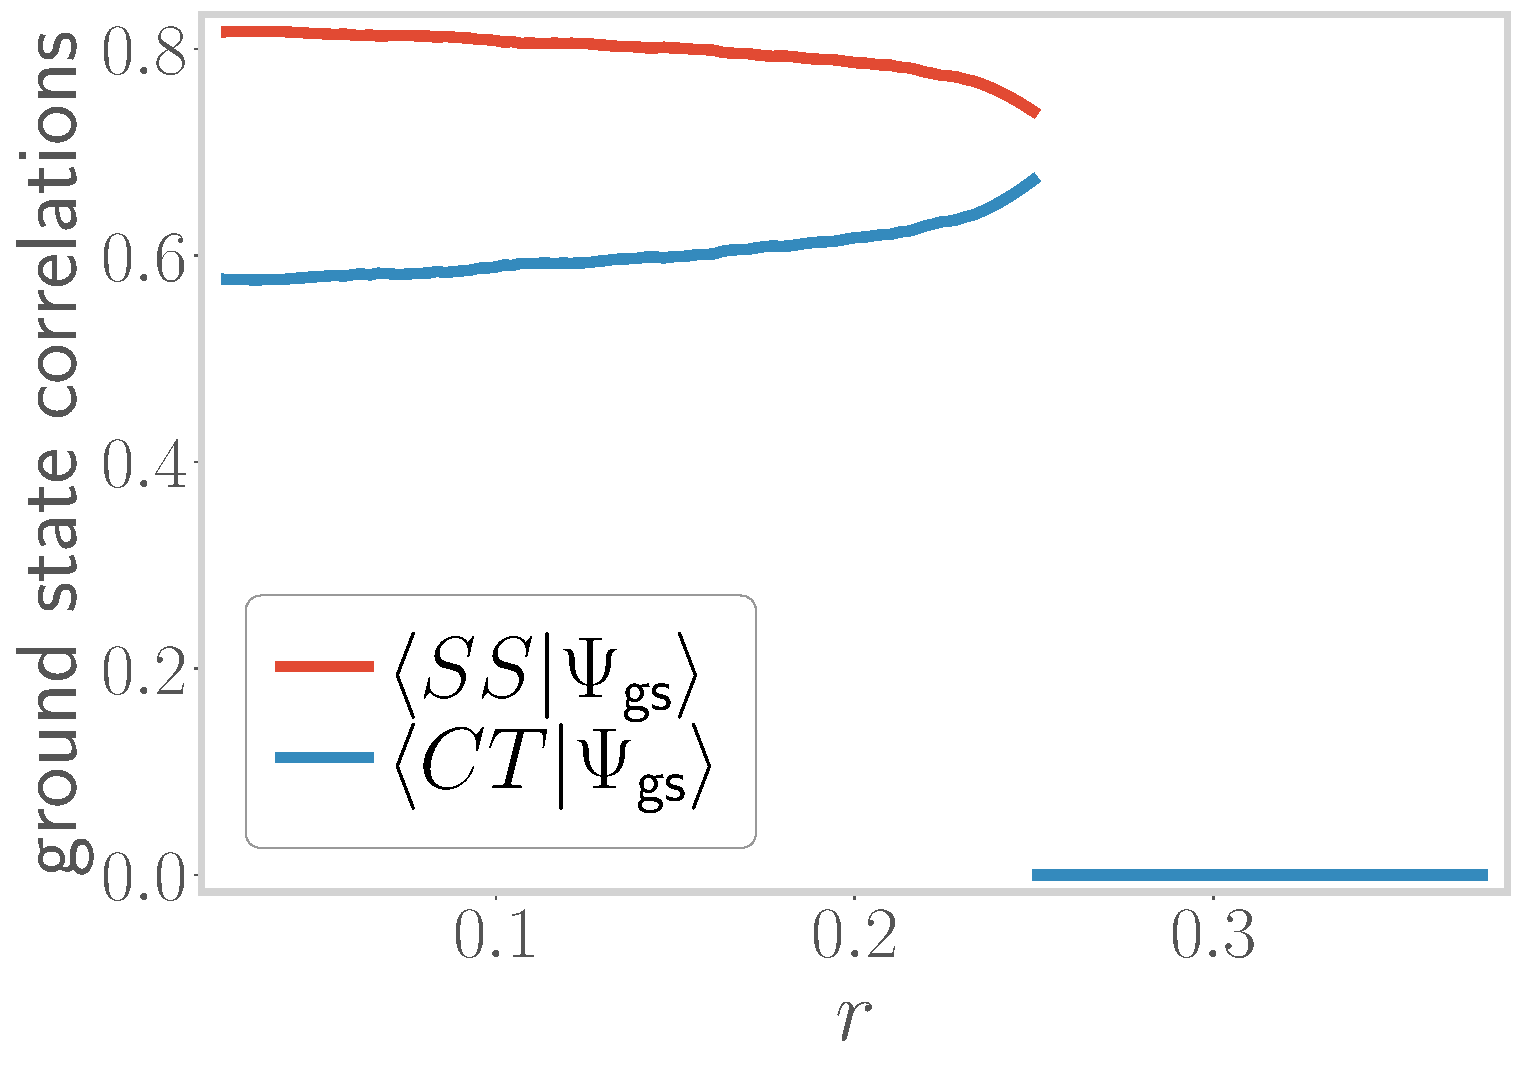
\includegraphics[width=0.99\textwidth]{figures/corrs_gs.pdf}

\end{minipage}

\vspace*{20pt}

ground state has both \focus{spin} and \focus{charge} entanglement

\end{frame}

\section{Descriptors of the transition}
\begin{frame}{Spectral function:~ ~ Transfer of spectral weight along the transition}
\hspace*{-45pt}
\begin{minipage}{0.5\textwidth}
	\begin{itemize}
		\item single peak at \(r \ll 1/4\), side peaks appear for \(r \simeq 1/4\)\\[20pt]
		\item gap appears for \(r > 1/4\)\\[20pt]
 		\item pole in impurity Greens function is replaced by a zero
	\end{itemize}
\end{minipage}
\begin{minipage}{0.49\textwidth}
	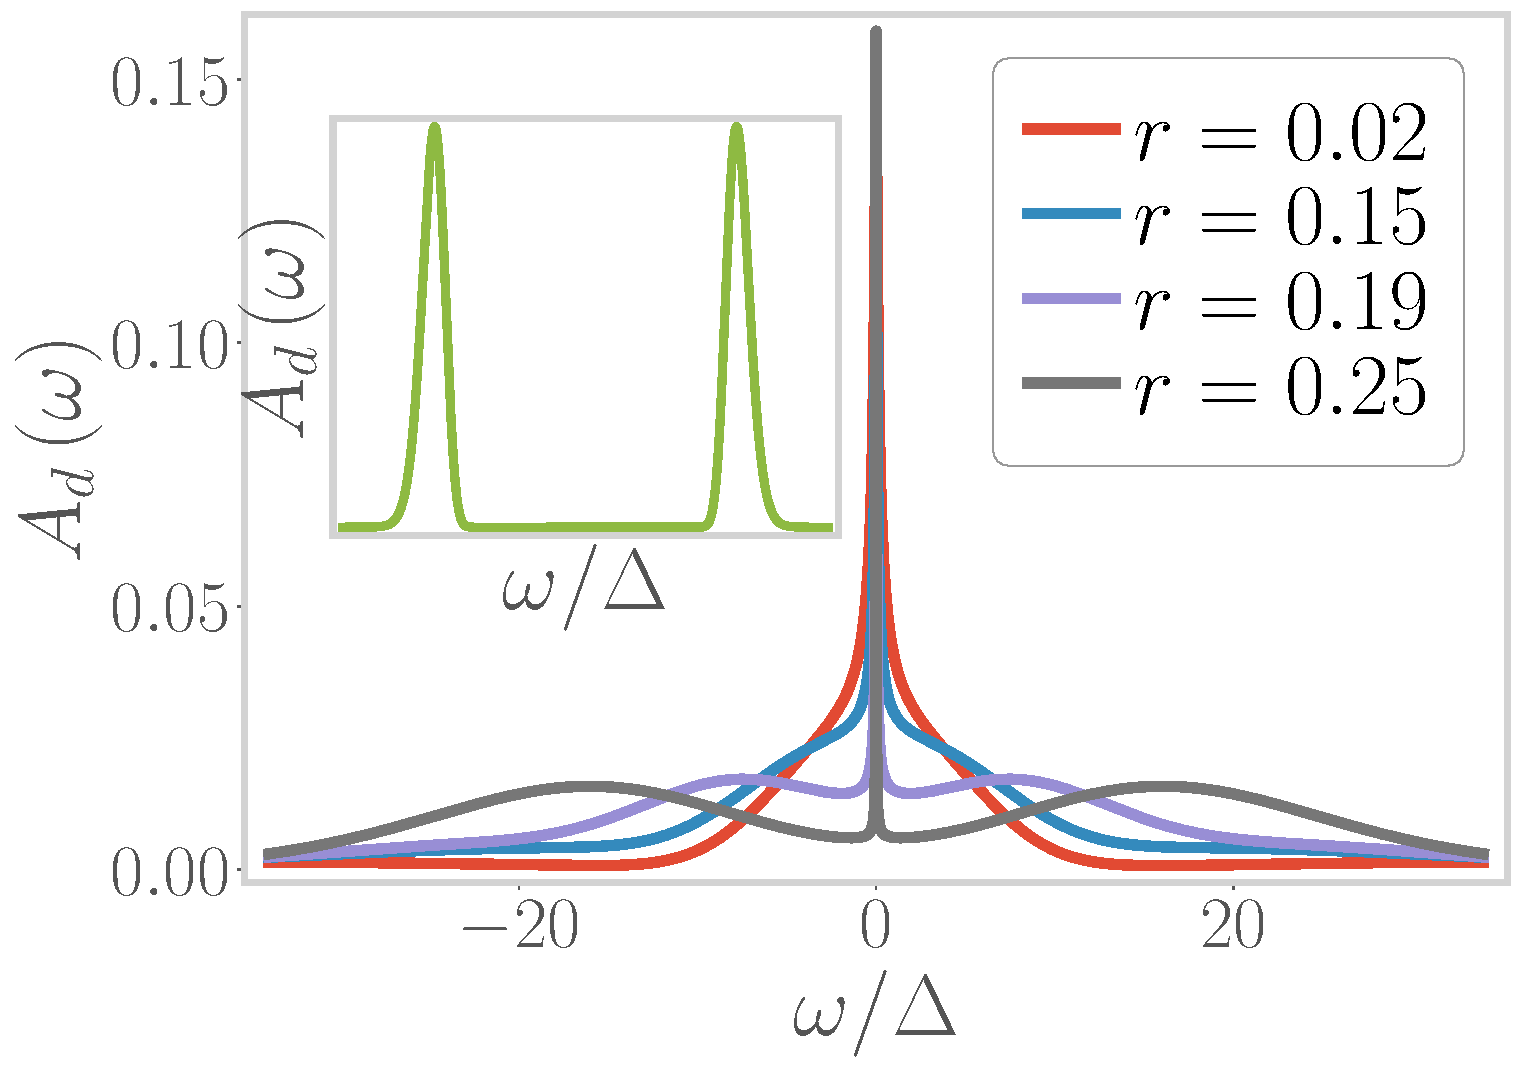
\includegraphics[width=1.2\textwidth]{figures/Add.pdf}
\end{minipage}

\footcite{hewson1993}
\end{frame}

\begin{frame}{Geometric entanglement as an order parameter for the transition}

	\focus{Geometric entanglement}: \(\varepsilon\left(\psi_1,\psi_2\right) = 1 - |\braket{\psi_1 | \psi_2}|^2\)\\[20pt]

	\(\ket{\Psi}_\text{gs} \simeq \ket{\Phi}_{ss}\braket{\text{ss}|\Psi^{(2)}_\text{gs}} + \ket{\Phi}_{ct}\braket{\text{ct}|\Psi^{(2)}_\text{gs}}\)\\[20pt]

	\(G_d(\omega) = \left(1 - \varepsilon_\text{ss} \right) \mathcal{G}_\text{ss} + \left(1 - \varepsilon_\text{ct} \right) \mathcal{G}_\text{ct} + \sqrt{\left(1 - \varepsilon_\text{ss} \right)}\sqrt{\left(1 - \varepsilon_\text{ct} \right)} \mathcal{G}_\text{ss-ct}\)\\[20pt]

	\(\longrightarrow~\)\focus{\bf relates} Green functions to a measure of entanglement

	\footcite{shimony1995degree,wei2003geometric,horodecki2009quantum}
\end{frame}

\begin{frame}{Geometric entanglement as an order parameter for the transition}

\hspace*{-10pt}
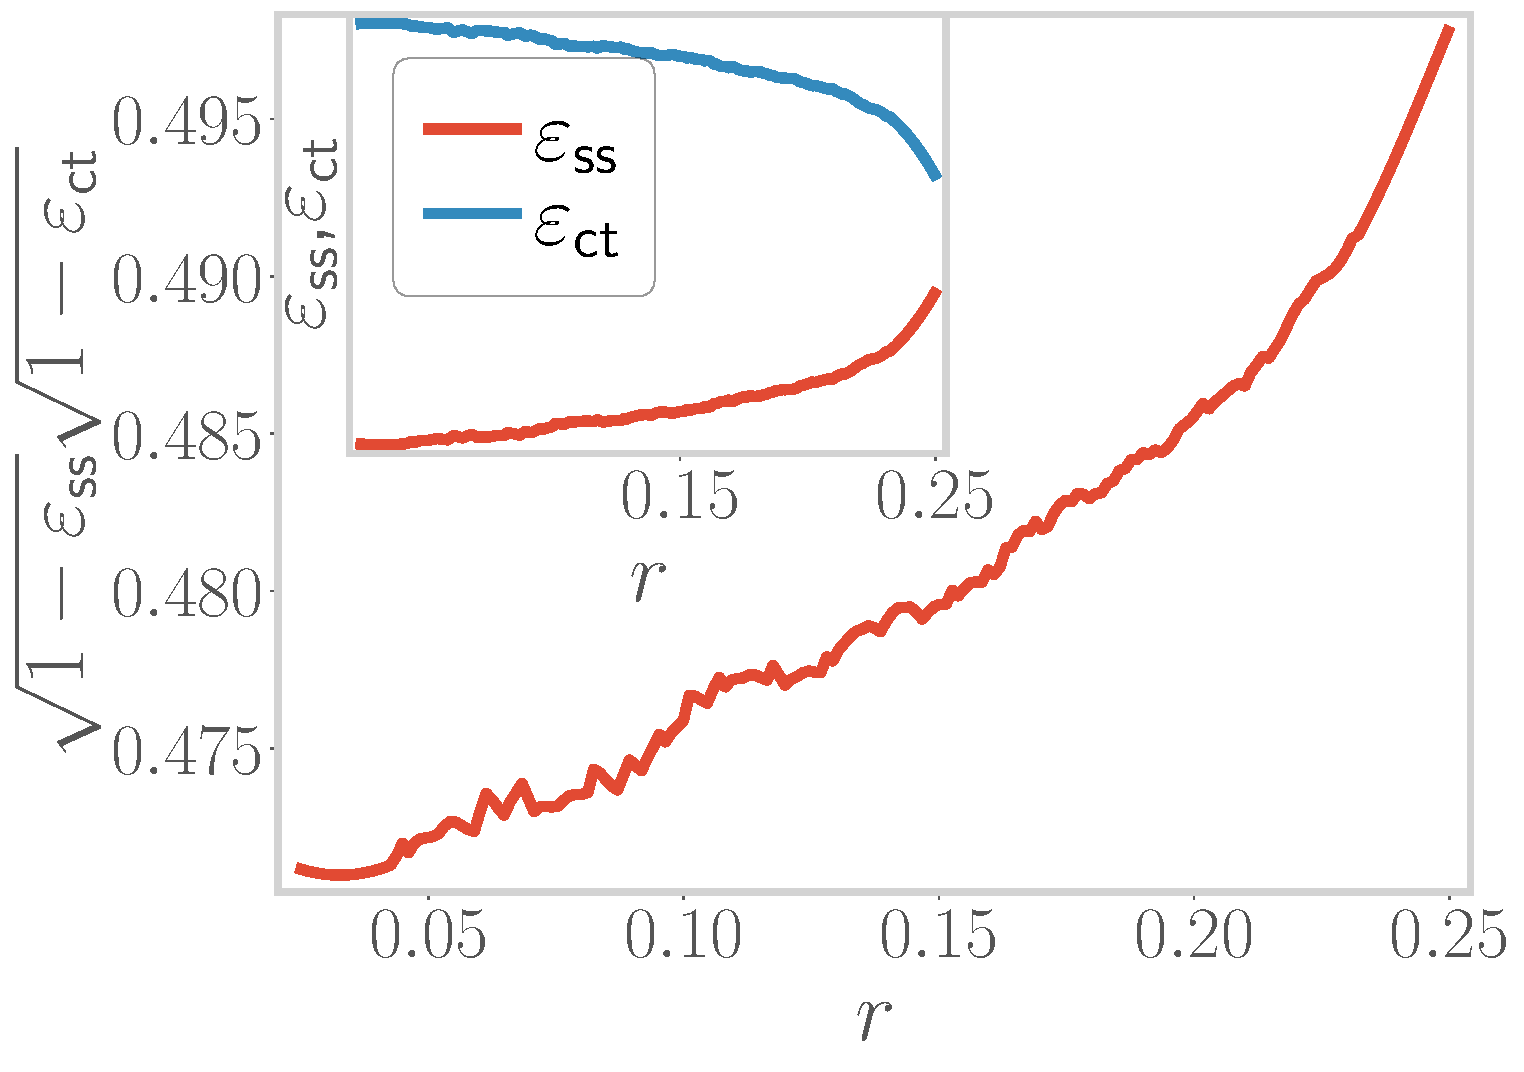
\includegraphics[width=0.49\textwidth]{figures/entanglement.pdf}
\hspace*{\fill}
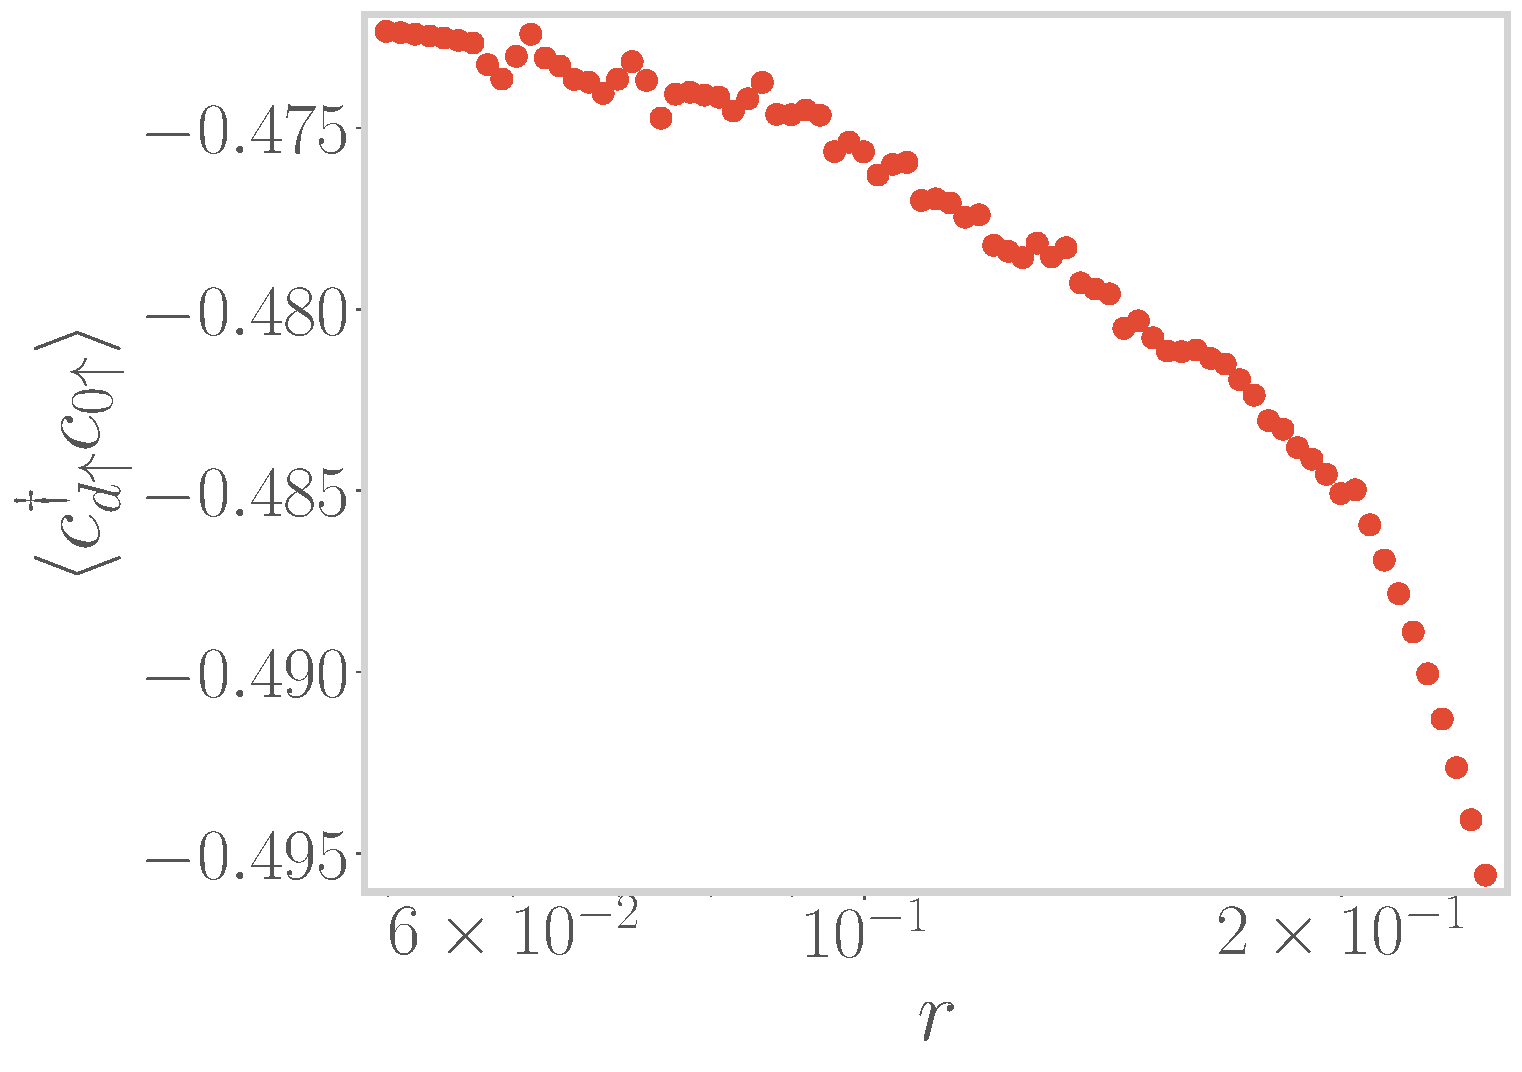
\includegraphics[width=0.49\textwidth]{figures/corr_1p.pdf}

\begin{itemize}
	\item Entanglement of spin increases towards the transition, that of charge decreases \\[10pt]
	\item Cross-term \(\sqrt{\left(1 - \varepsilon_\text{ss} \right)}\sqrt{\left(1 - \varepsilon_\text{ct} \right)}\) has an overall increase\\[10pt]
	\item Increased \focus{mixing between spin and charge} sectors (through 1-particle terms)
\end{itemize}

\end{frame}

\begin{frame}{Geometric entanglement as an order parameter for the transition}

	For \focus{general} \(T=0\) static correlation \(\left<O_2 O_1^\dagger \right>\):
	\[\left<O_2 O_1^\dagger\right> = \left(1 - \varepsilon_\text{ss}\right) \braket{O_2 O_1^\dagger}_\text{ss} + \left(1 - \varepsilon_\text{ct}\right) \braket{O_2 O_1^\dagger}_\text{ct} + \sqrt{1 - \varepsilon_\text{ss}}\sqrt{1 - \varepsilon_\text{ct}}\braket{O_2 O_1^\dagger}_\text{ss-ct}\]

\begin{minipage}{0.5\textwidth}
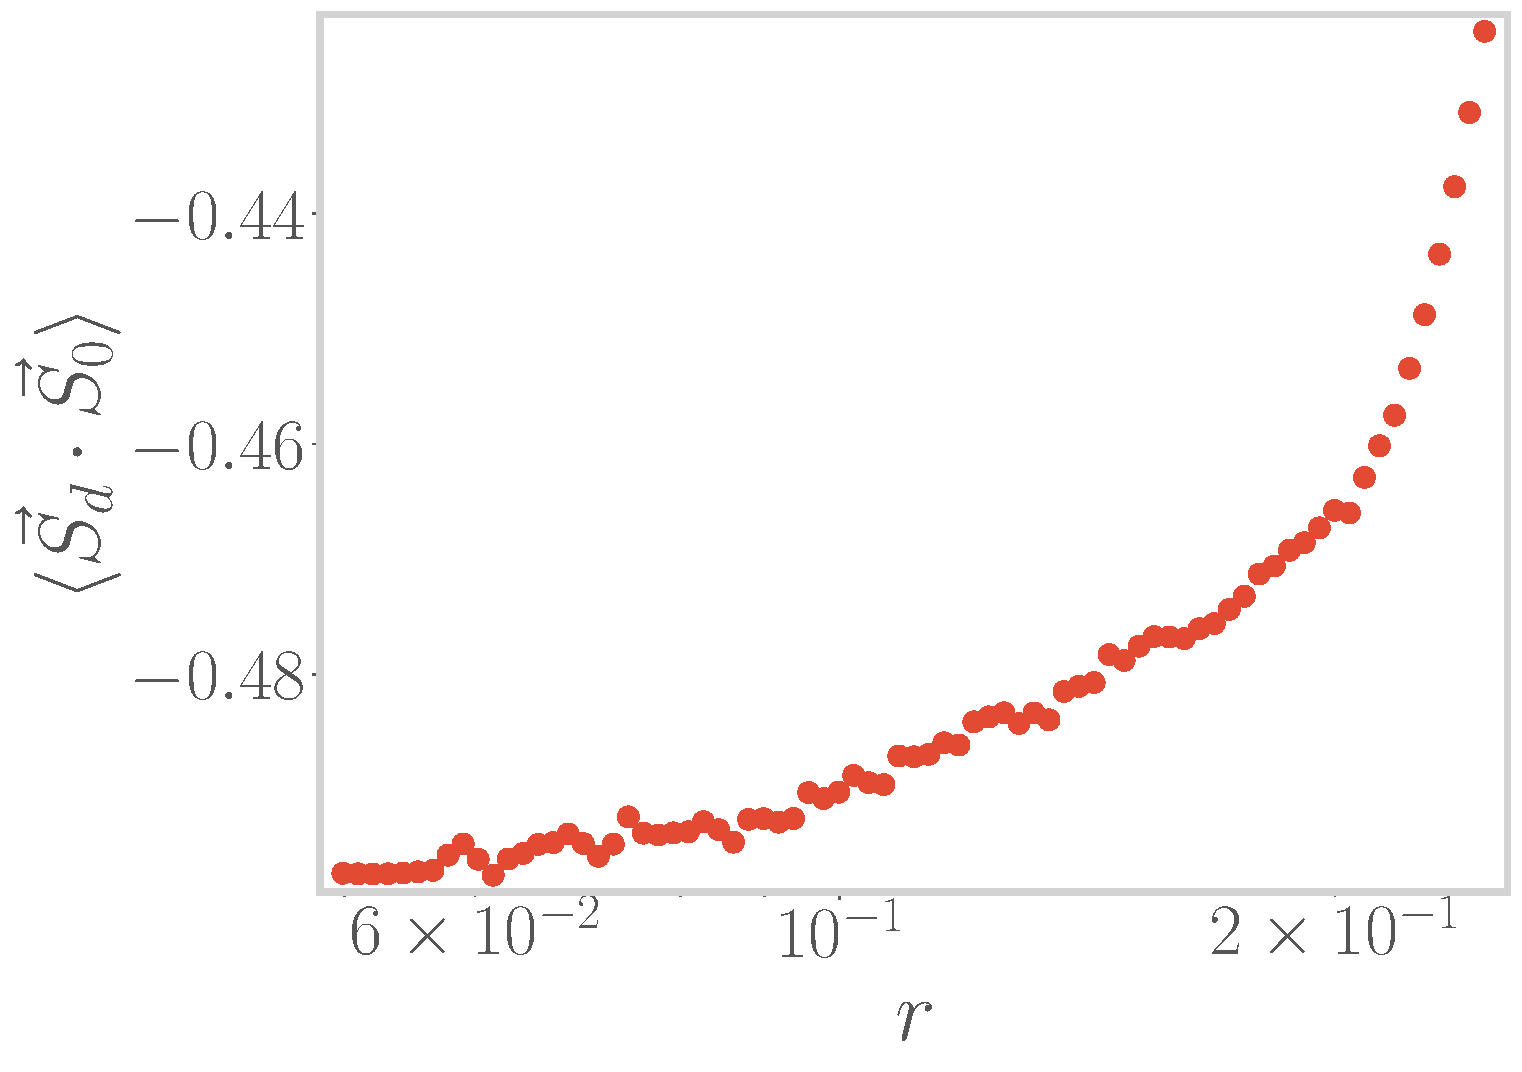
\includegraphics[width=0.99\textwidth]{figures/compens.pdf}
\end{minipage}
\begin{minipage}{0.49\textwidth}
	\begin{itemize}
		\item compensation depends only on \(\varepsilon_\text{ss}\)\\[20pt]
		\item \(\varepsilon_\text{ss}\) decreases towards transition\\[20pt]
		\item explains increase in compensation
	\end{itemize}
\end{minipage}

\vspace*{\fill}

\end{frame}

\begin{frame}{Mutual information \& spin-charge correlations: Fate of the Kondo cloud}

\begin{itemize}
\item \(\text{ground state \focus{density matrix}:~ ~}\rho = \ket{\Psi_\text{gs}}\bra{\Psi_\text{gs}}\)\\[20pt]
\item \(\text{reduced density matrix - \focus{trace out} certain DOFs~: ~ ~}\rho_A = \text{Tr}_A\left[\rho\right]\)\\[20pt]
\only<2>{
\item \(\text{\focus{entanglement entropy} of A w.r.t. rest:~ ~}S(A) = -\text{Tr}\left[\rho_A \ln \rho_A\right]\)\\[20pt]
\item \(\text{\focus{mutual information} between A and B:~ ~}I(A:B) = S(A) + S(B) - S(A \cup B)\)
}
\end{itemize}

\end{frame}

\begin{frame}{Mutual information \& spin-charge correlations: Fate of the Kondo cloud}

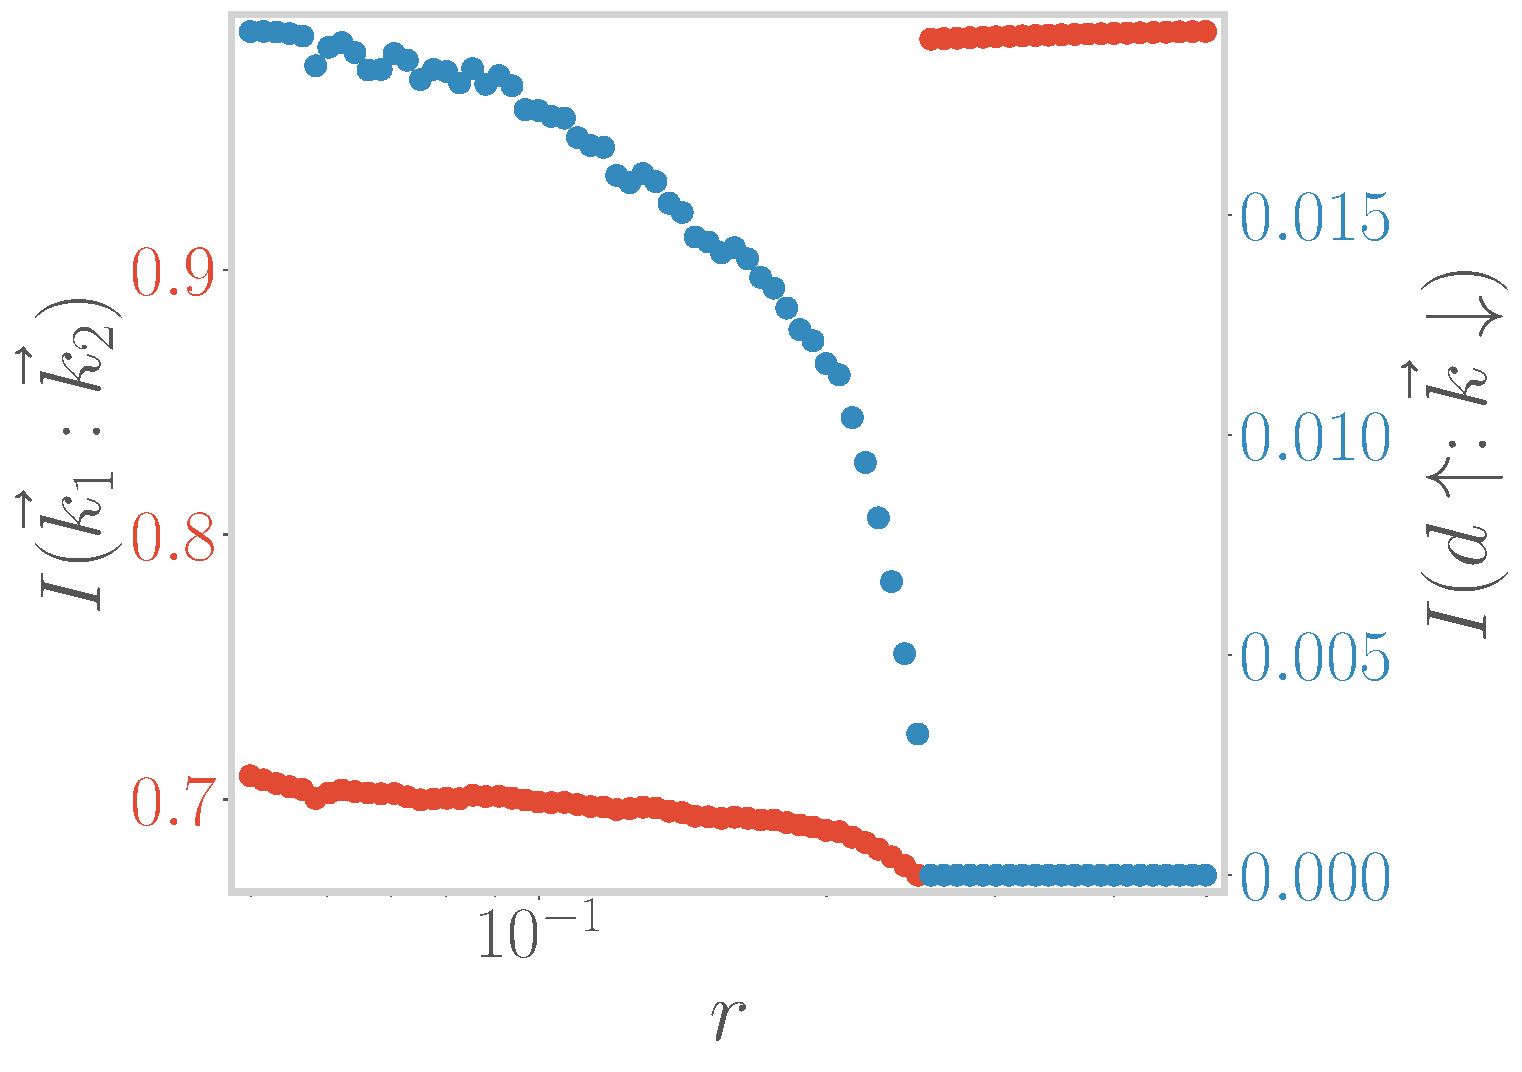
\includegraphics[width=0.5\textwidth]{figures/I_k.pdf}

\vspace*{10pt}

\begin{itemize}
\item MI within Kondo cloud as well as between impurity and \(k-\)states decreases\\[10pt]
\item signature of \focus{destruction of the Kondo cloud}\\[10pt]
\item beyond the transition, \(I(d:k) \) drops to zero, while \(I(k:k^\prime)\) rises

\end{itemize}

\end{frame}

\begin{frame}{Mutual information \& spin-charge correlations: Fate of the Kondo cloud}

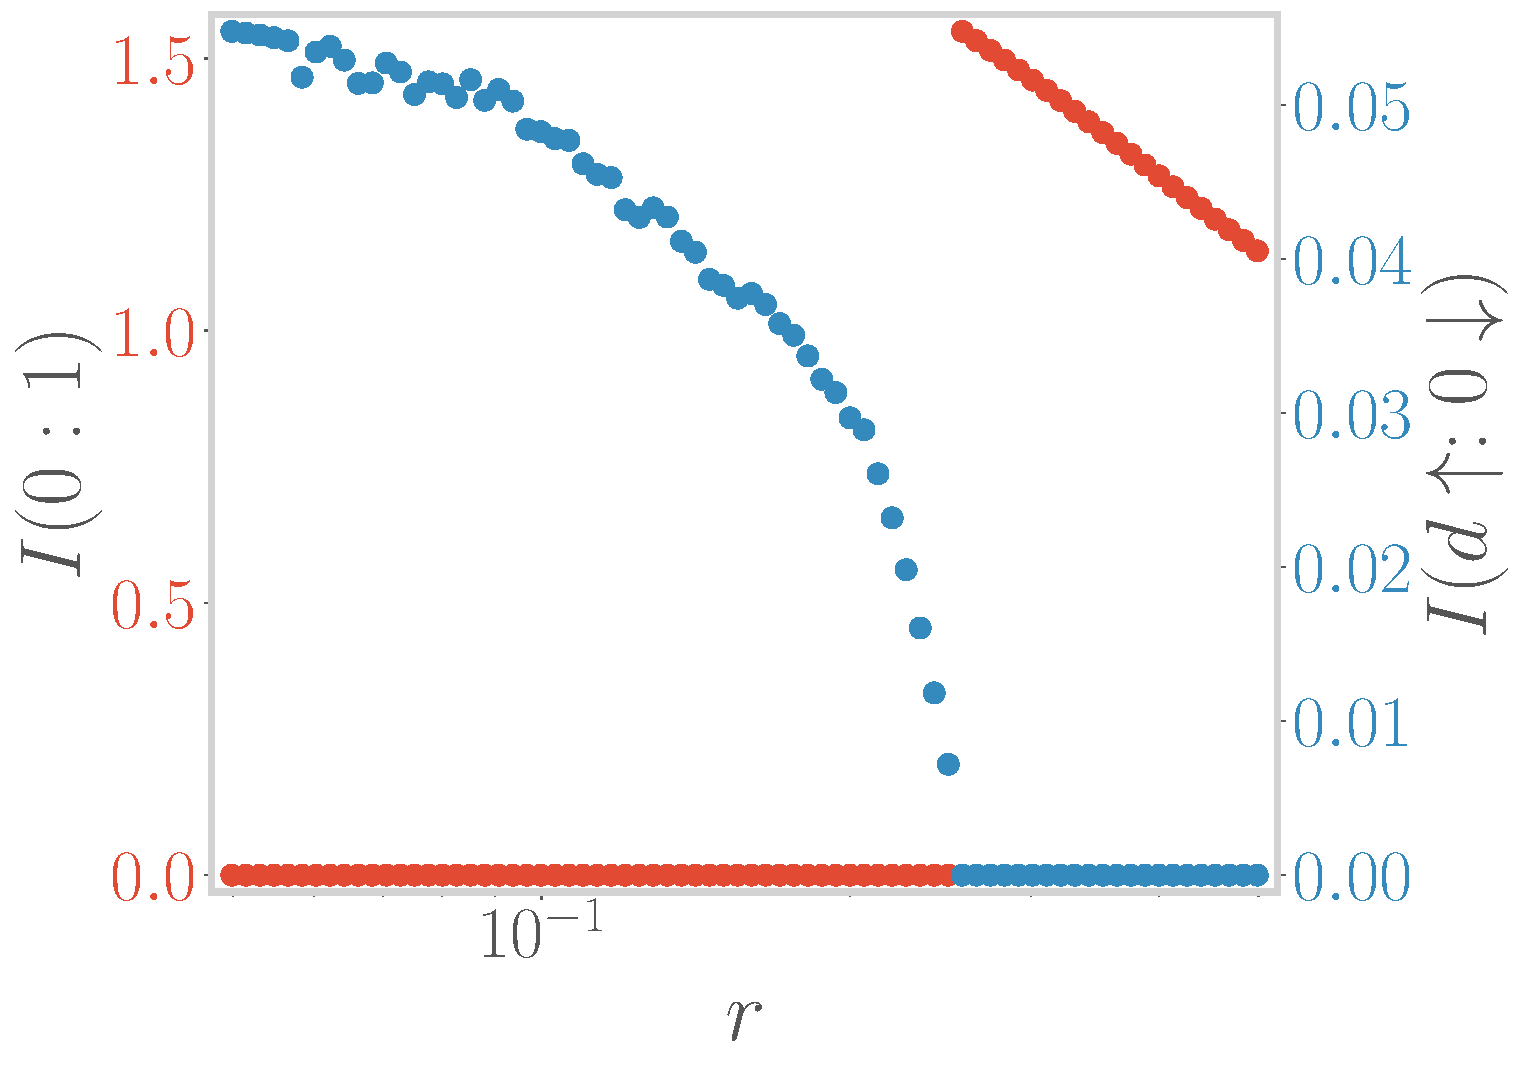
\includegraphics[width=0.5\textwidth]{figures/I_r.pdf}

\vspace*{10pt}

\begin{itemize}
	\item in real-space, impurity-zeroth site \focus{singlet} gets decoupled into \focus{separable} state\\[10pt]
\item this entanglement is transferred inot \(0:1\) system\\[10pt]
\item shows the \focus{redistribution of entanglement} from impurity site to the lattice
\end{itemize}

\end{frame}

\begin{frame}{Mutual information \& spin-charge correlations: Fate of the Kondo cloud}

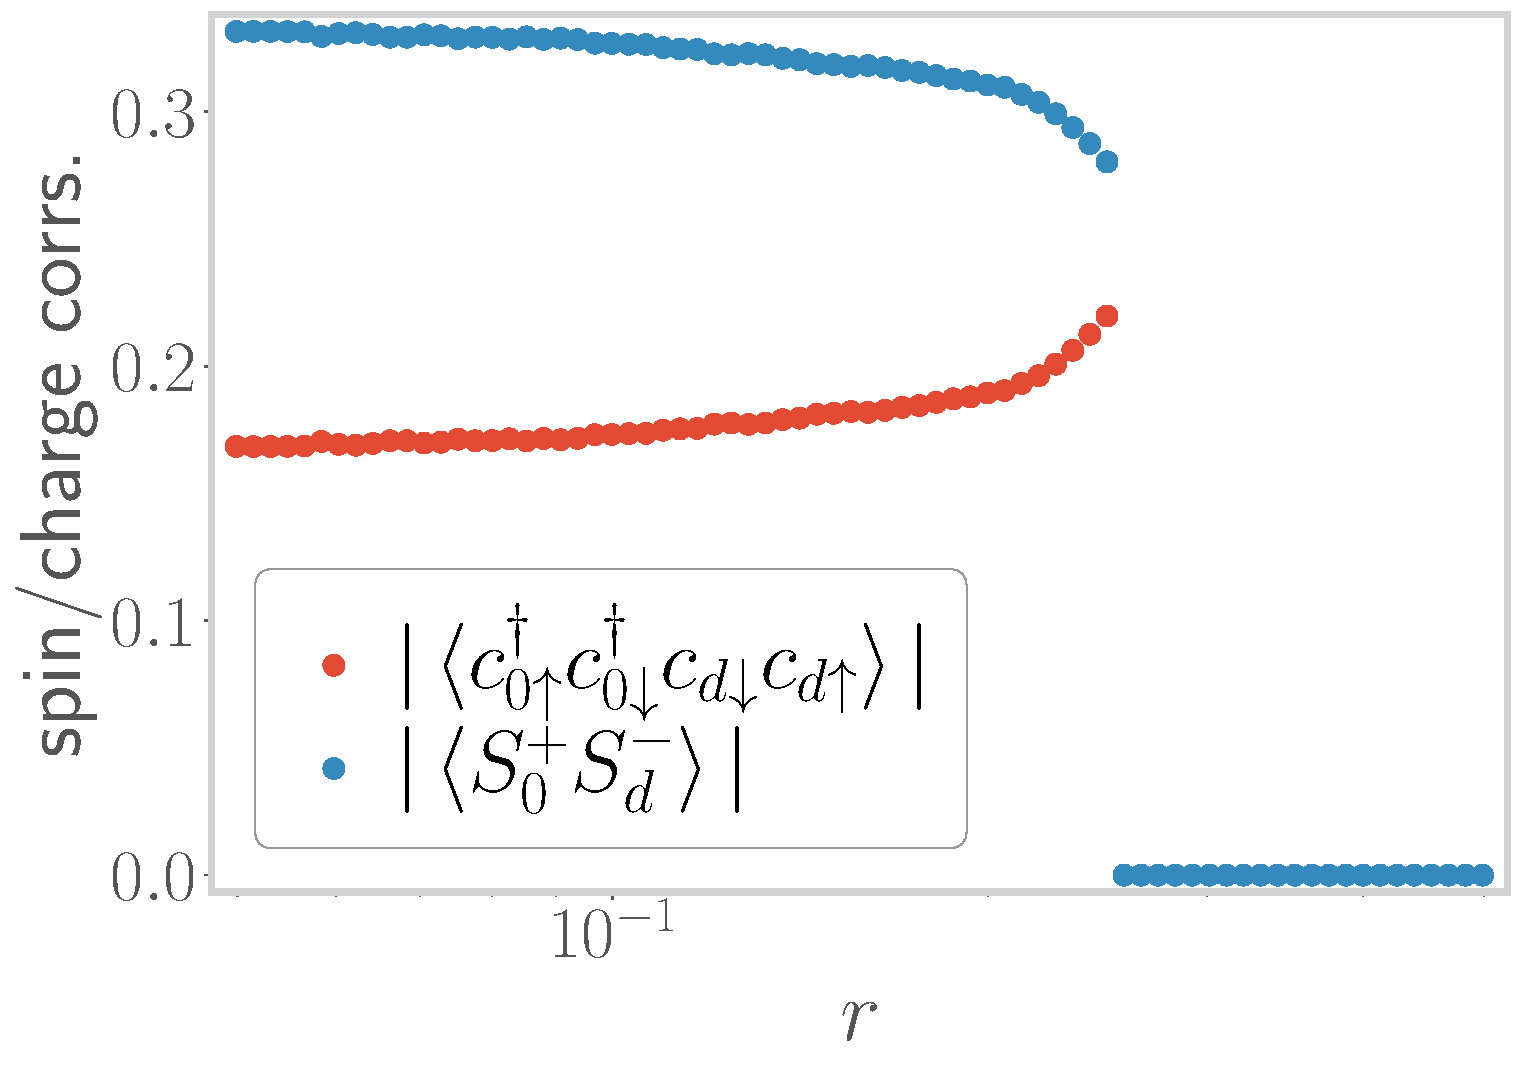
\includegraphics[width=0.5\textwidth]{figures/odlro_d0.pdf}

\vspace*{10pt}

\begin{itemize}
	\item lowering of spin-fluctuations explains destruction of Kondo cloud\\[10pt]
\item attractive \(U_b\) leads to pair-fluctuations between impurity and zeroth site
\end{itemize}

\end{frame}


\section{Final Remarks}
\label{concl}

\begin{frame}{Conclusions and Insights}
\begin{itemize}
	\item \(J\) and \(U_b\) lead to \focus{multiple phases} under RG, with distinct eff. Hamiltonians and g.states\\[20pt]
	\item Presence of \focus{subdominant pair fluctuations} between \(d\) and 0 : reminiscent of subdominant \focus{Cooper-pairing tendency} in URG study of \(\mu=0\) Hubbard model\\[20pt]
	\item \(\chi = \sqrt{1-\varepsilon_\text{ss}}\sqrt{1-\varepsilon_\text{ct}}\) is non-zero in screened phase and 0 in unscreened phase: acts as \focus{order parameter} for the transition\\[20pt]
	\item Discontinuous change in \(\chi\) across the transition linked to the change in the topological Luttinger volume
\end{itemize}
\end{frame}

\begin{frame}{Moving forward}
\begin{itemize}
	\item Changing the filling might lead to \focus{dominant fluctuations} in pair formation\\[20pt]
	\item \(k-\)space \focus{geometry effects} can be captured by considering more impurities\\[20pt]
	\item Restoring translation invariance using an appropriate translation algorithm can promote this local MIT to a \focus{bulk transition}
\end{itemize}
\end{frame}

\begin{frame}[allowframebreaks]{References}
\printbibliography
\end{frame}

\end{document}
